%!TEX root = ../T1_Gomez_Luis_.tex

\chapter{Ensayos y resultados} % Main chapter title
\label{Chapter4} % For referencing this chapter elsewhere, use \ref{Chapter4}

%----------------------------------------------------------------------------------------
%	SECTION 1
%----------------------------------------------------------------------------------------

Este capítulo presenta la evaluación del sistema de medición de \MPF desarrollado, abarcando validación técnica, caracterización metrológica y rendimiento operativo. Se analizaron los resultados de las pruebas realizadas sobre el diseño electrónico, el sistema de alimentación y la implementación del software mediante un banco de pruebas estructurado. Se evalúa la calidad metrológica del instrumento a través del análisis de correlación entre los tres sensores redundantes y su comparación con equipos de referencia. La caracterización operativa incluye la verificación de la completitud de datos adquiridos, el análisis de patrones temporales de concentración, y la respuesta del instrumento ante un evento controlado de alta contaminación. Los resultados obtenidos, presentados mediante análisis estadístico y visualizaciones temporales, muestran que el sistema alcanza los niveles de confiabilidad y precisión requeridos para aplicaciones de monitoreo ambiental urbano.

\section{Banco de prueba} 


%	1	Descripción de las herramientas utilizadas para probar el dispositivo	Imágenes de equipos de prueba	Métodos de prueba y sus parámetros


El banco de pruebas se estructuró en cuatro categorías funcionales complementarias: instrumentación electrónica, validación metrológica, verificación de hardware y pruebas de software.

La instrumentación electrónica comprendió equipos para la caracterización y diagnóstico de los circuitos. Se utilizó un analizador lógico de \SI{24}{\mega\hertz} con 8 canales para la verificación de protocolos de comunicación (\IIC, SPI, UART), lo que permitió monitorizar en tiempo real las transacciones de datos entre el microcontrolador y los periféricos. Para el análisis de señales de alta frecuencia, se empleó un osciloscopio FNIRSI1014D de \SI{100}{\mega\hertz}, que facilitó la medición de tiempos de respuesta, detección de interferencias y verificación de integridad de señales críticas. Las mediciones de parámetros eléctricos se realizaron con un multímetro digital TMT460012, con resolución de \SI{0.01}{\milli\volt} para tensión y \SI{0.1}{\micro\ampere} para corriente. La alimentación controlada del sistema durante las pruebas se implementó mediante una fuente regulada Jesverty SPS-3005 con rango de \SIrange{0}{30}{\volt} y capacidad de corriente de \SI{5}{\ampere}.

Para la validación metrológica, las mediciones de \MPF se contrastaron con un instrumento de referencia Grimm y equipo certificado por su alta precisión (\SI{\pm2}{\percent}) en el análisis óptico de partículas atmosféricas dentro del rango de \SIrange{0.3}{10}{\micro\meter}. Esta comparación se realizó en dos escenarios: bajo condiciones controladas de laboratorio y en ambiente real, lo que expone a los sensores a las condiciones atmosféricas urbanas durante un período de 72 horas. Este enfoque dual permitió determinar tanto la exactitud y precisión del instrumento como su comportamiento en condiciones operativas reales.

La verificación del hardware se efectuó mediante un proceso sistemático que incluyó la comprobación del cumplimiento de las reglas de diseño de circuito impreso utilizó las herramientas integradas en KiCad. Este proceso verificó parámetros críticos como anchos de pista, distancias mínimas entre elementos y diámetros de vías. Adicionalmente, componentes  como inductores, capacitores y resistencias se caracterizaron individualmente con un medidor LCR-P1 de FNIRSI, que proporcionó datos  sobre sus propiedades eléctricas y tolerancias reales, lo que permite validar que sus valores se encontraban dentro de los márgenes establecidos para garantizar el funcionamiento correcto del circuito.

Las pruebas de software implementaron metodologías de validación mediante el framework Ceedling, que permitió la automatización de pruebas unitarias en lenguaje C. Esta aproximación posibilitó la evaluación independiente de cada módulo del firmware, facilitó la detección temprana de errores lógicos o de implementación. La integración de las herramientas Unity y CMock dentro del framework proporcionó capacidades para la creación de objetos simulados (\textit{mocks}) y aserciones específicas para validar el comportamiento esperado de las funciones. La verificación de comunicaciones se complementó con un terminal UART Cutecom, configurado a \SI{115200}{\baud}, para la inspección detallada de los datos transmitidos entre el sistema y los dispositivos periféricos, lo que facilitó la verificación del cumplimiento de los protocolos establecidos.

Las tablas \ref{tab:pruebas} y  \ref{tab:pruebas2} presentan un resumen  de los instrumentos empleados en el banco de pruebas. Esta detalla las características técnicas y función específica en el proceso de validación.





%\section{Pruebas funcionales del hardware}
%\label{sec:pruebasHW}

%La idea de esta sección es explicar cómo se hicieron los ensayos, qué resultados se obtuvieron y analizarlos.




\section{Evaluación del software}
%	3	Evaluación del rendimiento del hardware y herramientas empleadas para su evaluación	Fotos del prototipo final	Tabla con herramientas empleadas


La validación del sistema de medición de \MPF se enfocó en garantizar la precisión y confiabilidad del subsistema de análisis, identificado como componente crítico con una importancia relativa del 24\% según los criterios de diseño establecidos. Este componente procesa los datos provenientes de los sensores ópticos y realiza los cálculos estadísticos necesarios para determinar las concentraciones del contaminante.

\subsection{Metodología de pruebas de software}

Se implementó el \textit{Método del Árbol de Clasificación} (CTM) como estrategia principal para el diseño y ejecución de los casos de prueba. Esta técnica permitió una cobertura  y sistemática de los posibles escenarios de operación, lo que facilita la identificación de errores potenciales en el tratamiento de datos. El proceso consistió en cuatro etapas secuenciales:

\begin{enumerate}
	\item Definición de clases de equivalencia: se estableció categorías para los tipos de datos de entrada, lo que incluyó concentraciones dentro de los límites operativos (\SIrange{0.5}{500}{\micro\gram\per\cubic\meter}), valores por debajo del límite mínimo de cuantificación, mediciones que exceden el límite máximo de linealidad y casos atípicos como valores negativos o nulos.
	
	\item Construcción del árbol de clasificación: se desarrolló una estructura jerárquica que representa las diferentes clases de equivalencia y las relaciones entre ellas, lo que permitió la identificación de combinaciones específicas de condiciones para cada caso de prueba.
	
	\item Derivación de casos de prueba: a partir del árbol de clasificación, se identificó cinco escenarios representativos que abarcan las principales condiciones de operación y casos límite del sistema.
	
	\item Ejecución y análisis de resultados: se utilizó el framework Ceedling, junto con las herramientas Unity y CMock, para implementar y automatizar la ejecución de las pruebas unitarias.
\end{enumerate}

\subsection{Casos de prueba implementados}

Se desarrollaron cinco casos  para evaluar la función \texttt{calculateAverage} de la API \texttt{ParticulateDataAnalyzer}, responsable del cálculo del promedio de concentraciones de MP$_{2,5}$ bajo diferentes condiciones:

\begin{table}[h]
	\centering
	\small
	\caption{Resumen de los casos de prueba aplicados al subsistema de análisis.}
	\label{tab:casos-prueba-software}
	\begin{tabular}{c p{4.5cm} p{4.5cm} c }
		\hline
		\textbf{Test} & \textbf{Escenario} & \textbf{Objetivo} & \textbf{Resultado} \\
		\hline
		1 & Valores dentro del rango con algunos por debajo del límite de cuantificación & Verificar exclusión correcta de valores $< \SI{0.5}{\micro\gram\per\cubic\meter}$ & \SI{302.5}{\micro\gram\per\cubic\meter} \\
		
		2 & Datos válidos con algunos valores por encima del máximo y negativos & Comprobar manejo adecuado de valores fuera de rango superior y negativos & \SI{286.07}{\micro\gram\per\cubic\meter} \\
		
		3 & Arreglo completo de datos nulos & Validar respuesta ante ausencia total de datos válidos & $-999$ \\
		
		4 & Todos los valores dentro del rango permitido & Confirmar cálculo correcto con datos completamente válidos & \SI{316.67}{\micro\gram\per\cubic\meter} \\
		
		5 & Arreglo sin datos válidos (todos bajo límite) & Verificar comportamiento con datos insuficientes para cálculo & $-999$ \\
		\hline
	\end{tabular}
\end{table}

El caso de prueba 1 evaluó el procesamiento de un conjunto de datos donde la mayoría se encontraba dentro del rango operativo, lo que incluyó valores ligeramente por debajo del límite inferior de cuantificación (\SI{0.4}{\micro\gram\per\cubic\meter} y \SI{0.3}{\micro\gram\per\cubic\meter}). Esta prueba verificó que el sistema excluyera correctamente estos valores del cálculo del promedio y utilizara solo los 16 valores válidos restantes.

El caso 2 analizó el manejo de valores extremos, lo que incorporó tanto concentraciones negativas (\SI{-480}{\micro\gram\per\cubic\meter}) como mediciones superiores al límite máximo de linealidad (\SI{590}{\micro\gram\per\cubic\meter} y \SI{895}{\micro\gram\per\cubic\meter}). Esta prueba fue particularmente significativa para validar la robustez del sistema ante lecturas anómalas o errores de medición.

Los casos 3 y 5 evaluaron situaciones límite donde no existían datos válidos para el cálculo, ya sea por un arreglo completamente vacío o con datos por debajo del umbral mínimo de cuantificación. Ambos casos verificaron que el sistema respondiera adecuadamente con un valor de error predefinido ($-999$), lo que señaló la imposibilidad de realizar el cálculo.

El caso 4 representó un escenario ideal con todos los valores dentro del rango operativo permitido, lo que verificó la precisión del cálculo bajo condiciones óptimas de funcionamiento.

\subsection{Implementación de las pruebas}

Las pruebas se codificaron con el framework Ceedling, que integra las herramientas Unity y CMock para la automatización de pruebas unitarias en lenguaje C (ver figura \ref{fig:resultados-pruebas}). Cada caso de prueba se implementó como una función independiente que preparaba los datos de entrada, ejecutaba la función bajo evaluación y verificaba que el resultado correspondiera al valor esperado mediante aserciones.

La función \texttt{calculateAverage} evaluada realiza el procesamiento de un arreglo de valores flotantes que representan concentraciones de \MPF, con los siguientes pasos:

\begin{enumerate}
	\item Verifica si el arreglo está vacío mediante la función \texttt{isArrayEmpty}.
	\item Inicializa variables para sumatoria y conteo de valores no válidos.
	\item Recorre cada elemento del arreglo, lo que validó cada valor mediante la función \texttt{maskIsDataTrue}.
	\item Para los valores válidos, acumula la suma; para los inválidos, incrementa el contador.
	\item Recalcula el número efectivo de datos válidos.
	\item Verifica que exista al menos un valor válido antes de realizar la división.
	\item Retorna el promedio calculado o un valor de error predefinido.
\end{enumerate}

\begin{figure}[h]
	\centering
	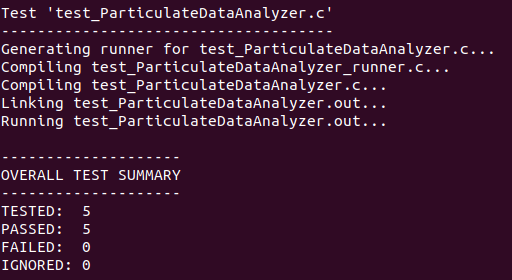
\includegraphics[width=0.7\linewidth]{Figures/captura_ceedling}
	\caption{Resultados de la ejecución de las pruebas unitarias mediante Ceedling.}
	\label{fig:resultados-pruebas}
\end{figure}

\subsection{Resultados y mejoras implementadas}

La ejecución de los casos de prueba permitió identificar un error en la implementación de la función \texttt{calculateAverage}, específicamente en la validación de valores por encima del límite máximo de linealidad. Este hallazgo permitió la corrección temprana de un problema que podría haber afectado el cálculo de los promedios de \MPF durante la operación del instrumento.

Tras la detección del error, se implementaron las siguientes mejoras:

\begin{itemize}
	\item Modificación de la función \texttt{maskIsDataTrue} para incorporar explícitamente la validación del límite superior de \SI{500}{\micro\gram\per\cubic\meter}.
	\item Refinamiento de la documentación del código para especificar claramente los rangos de valores aceptables.
	\item Incorporación de mensajes de error más descriptivos para facilitar la identificación de problemas en tiempo de ejecución.
	\item Optimización del algoritmo para mejorar el rendimiento en el procesamiento de grandes volúmenes de datos.
\end{itemize}

Los criterios de aceptación establecidos definieron una precisión con desviación estándar no superior al 5\% para el cálculo del promedio, requisito que fue verificado y cumplido mediante los casos de prueba implementados. Adicionalmente, se estableció un umbral mínimo del 75\% de datos válidos para considerar representativo un promedio horario, criterio que fue incorporado en la lógica de procesamiento y verificado mediante los casos de prueba.

La aplicación del MAT proporcionó un marco sistemático para diseñar, documentar y comunicar los casos de prueba. Esto aseguro la trazabilidad de los requisitos funcionales hasta su verificación final.	


\section{Pruebas de hardware}

Esta sección presenta los resultados de la evaluación de los componentes físicos del sistema de medición de \MPF. Se analizaron los resultados de la verificación del diseño electrónico, la caracterización individual de componentes críticos y las pruebas del sistema de alimentación. 

\subsection{Resultados del diseño electrónico}

La verificación del diseño electrónico  evaluó el cumplimiento de las reglas de diseño especificadas en las tablas \ref{tab:reglas_pcb} y \ref{tab:clases_redes} del Apéndice \ref{AppendixB}. Esta metodología integró herramientas de validación automática disponibles en KiCad 6.0 con inspección visual detallada, lo que permitió identificar y corregir discrepancias en parámetros críticos como anchos de pista (mínimo \SI{0.25}{\milli\meter} para señales, \SI{0.5}{\milli\meter} para potencia), distancias mínimas entre elementos (\SI{0.2}{\milli\meter}) y diámetros de vías (\SI{0.4}{\milli\meter} para señal, \SI{0.8}{\milli\meter} para potencia).

El diseño cumplió con las especificaciones técnicas establecidas en aproximadamente 90\% de la superficie de la PCB, a excepción de áreas específicas correspondientes al conector de memoria microSD y los circuitos integrados DS3231 y 74LVC125U8 (ver figura \ref{fig:pcbdetalle}). Para estos componentes de encapsulado predefinido fue necesario implementar zonas de exclusión de reglas de diseño, lo que redujo localmente la separación mínima a \SI{0.15}{\milli\meter} debido a las restricciones impuestas por su geometría de pines. Esta modificación  no comprometió la funcionalidad ni la fiabilidad del circuito. 

\begin{figure} [!hbp]
	\centering
	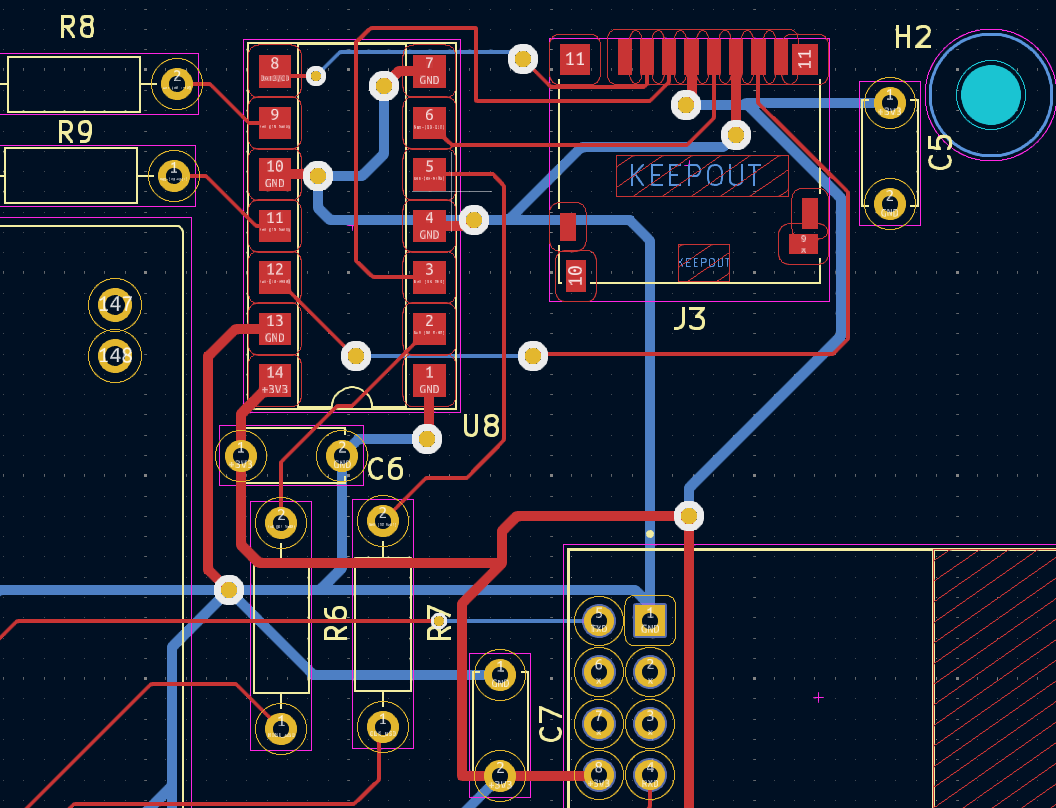
\includegraphics[width=0.7\linewidth]{Figures/PCB_detalle}
	\caption{Detalle de una sección  de la PCB donde se observan los anchos de pistas diferenciados para señal (\SI{0.25}{\milli\meter}) y potencia (\SI{0.5}{\milli\meter}), márgenes mínimos de separación y zonas de exclusión implementadas para los componentes de encapsulado predefinido.}
	\label{fig:pcbdetalle}
\end{figure}

El diseño incorporó además soluciones específicas para optimizar la manufactura y la integridad de señal, tales como alivios térmicos para pads de alta corriente, planos de tierra en capas internas para reducción de EMI, y pistas de impedancia controlada  para las líneas de comunicación críticas SPI y UART. Estas características de diseño, apreciables en la figura \ref{fig:detallepcb3d}, contribuyeron  a la robustez del sistema en términos de estabilidad eléctrica y resistencia a interferencias electromagnéticas externas, aspectos fundamentales para la precisión de las mediciones de \MPF.

\begin{figure} [!hbp]
	\centering
	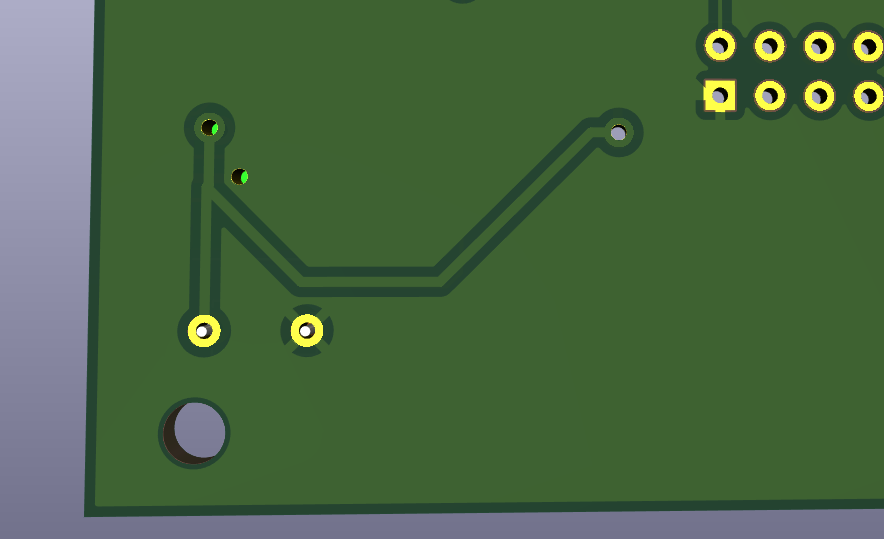
\includegraphics[width=0.7\linewidth]{Figures/Detalle_PCB_3D}
	\caption{Visualización de la PCB donde se aprecian los planos de tierra para reducción de interferencias (\SI{60}{\percent} de cobertura en capa superior), alivios térmicos para componentes de potencia, y vías  para estabilización de impedancia.}
	\label{fig:detallepcb3d}
\end{figure}


\newpage
\subsection{Verificación de componentes}

Previo a la integración del sistema completo, se realizó una etapa de verificación individualizada de cada componente crítico. Esta fase permitió detectar tempranamente posibles defectos y garantizar que todos los elementos cumplieran con las especificaciones técnicas requeridas. Se caracterizaron los componentes pasivos (resistencias, capacitores e inductores) mediante el medidor LCR-P1 de FNIRSI, lo que permite verificar sus valores nominales y tolerancias. Los sensores SPS30 fueron sometidos a pruebas funcionales en ambiente controlado para validar sus respuestas ópticas y calibración inicial. El microcontrolador STM32F429 y el módulo ESP8266 fueron verificados mediante pruebas de comunicación y respuesta a comandos específicos. Este proceso permitió asegurar la calidad individual de cada componente antes de su inclusión en el sistema integrado. Esta condición minimiza el riesgo de fallas durante la operación del instrumento.

\subsubsection{Resultados de la caracterización del sistema de alimentación}

Esta sección presenta los resultados obtenidos durante la evaluación del sistema de alimentación implementado para el instrumento de medición de \MPF. La caracterización se centró en los parámetros críticos para asegurar la precisión de las mediciones: estabilidad de tensión, nivel de ruido eléctrico y respuesta ante conmutaciones de fuente.

\subsubsection{Evaluación de componentes de ruido}

Los resultados de las pruebas iniciales con fuentes de alimentación convencionales mostraron niveles significativos de interferencia eléctrica, como se presenta en la figura \ref{fig:fuente_sin_filtro}. El análisis de estos datos reveló componentes de ruido con amplitudes de hasta \SI{78}{\milli\volt} pico-pico en frecuencias entre \SIrange{100}{150}{\kilo\hertz}.

\begin{figure}[h]
	\centering
	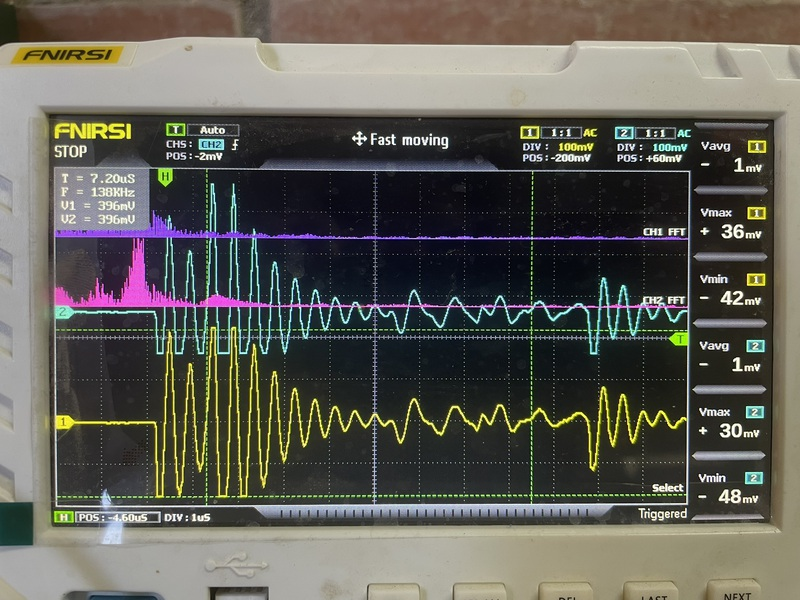
\includegraphics[width=0.8\linewidth]{Figures/test_fuente_condiciones_iniciales.JPEG}
	\caption{Registro de componentes de ruido en la fuente convencional con transitorios de alta frecuencia (\SI{138}{\kilo\hertz}) y amplitudes de aproximadamente \SI{78}{\milli\volt} pico-pico.}
	\label{fig:fuente_sin_filtro}
\end{figure}

Estas interferencias afectaron el funcionamiento de los sensores SPS30, cuya tecnología de dispersión láser presentó susceptibilidad a estas perturbaciones. El análisis estadístico confirmó correlación entre los eventos de ruido eléctrico y la aparición de valores atípicos en las mediciones de MP$_{2,5}$.

\subsubsection{Rendimiento del sistema de alimentación implementado}

El sistema jerárquico de alimentación con tres etapas (fuente primaria, módulo UPS y etapa de filtrado) mostró resultados satisfactorios en las pruebas de caracterización. La figura \ref{fig:modulo_ups} muestra el módulo UPS LX-28UPS utilizado en la implementación.

\begin{figure}[h]
	\centering
	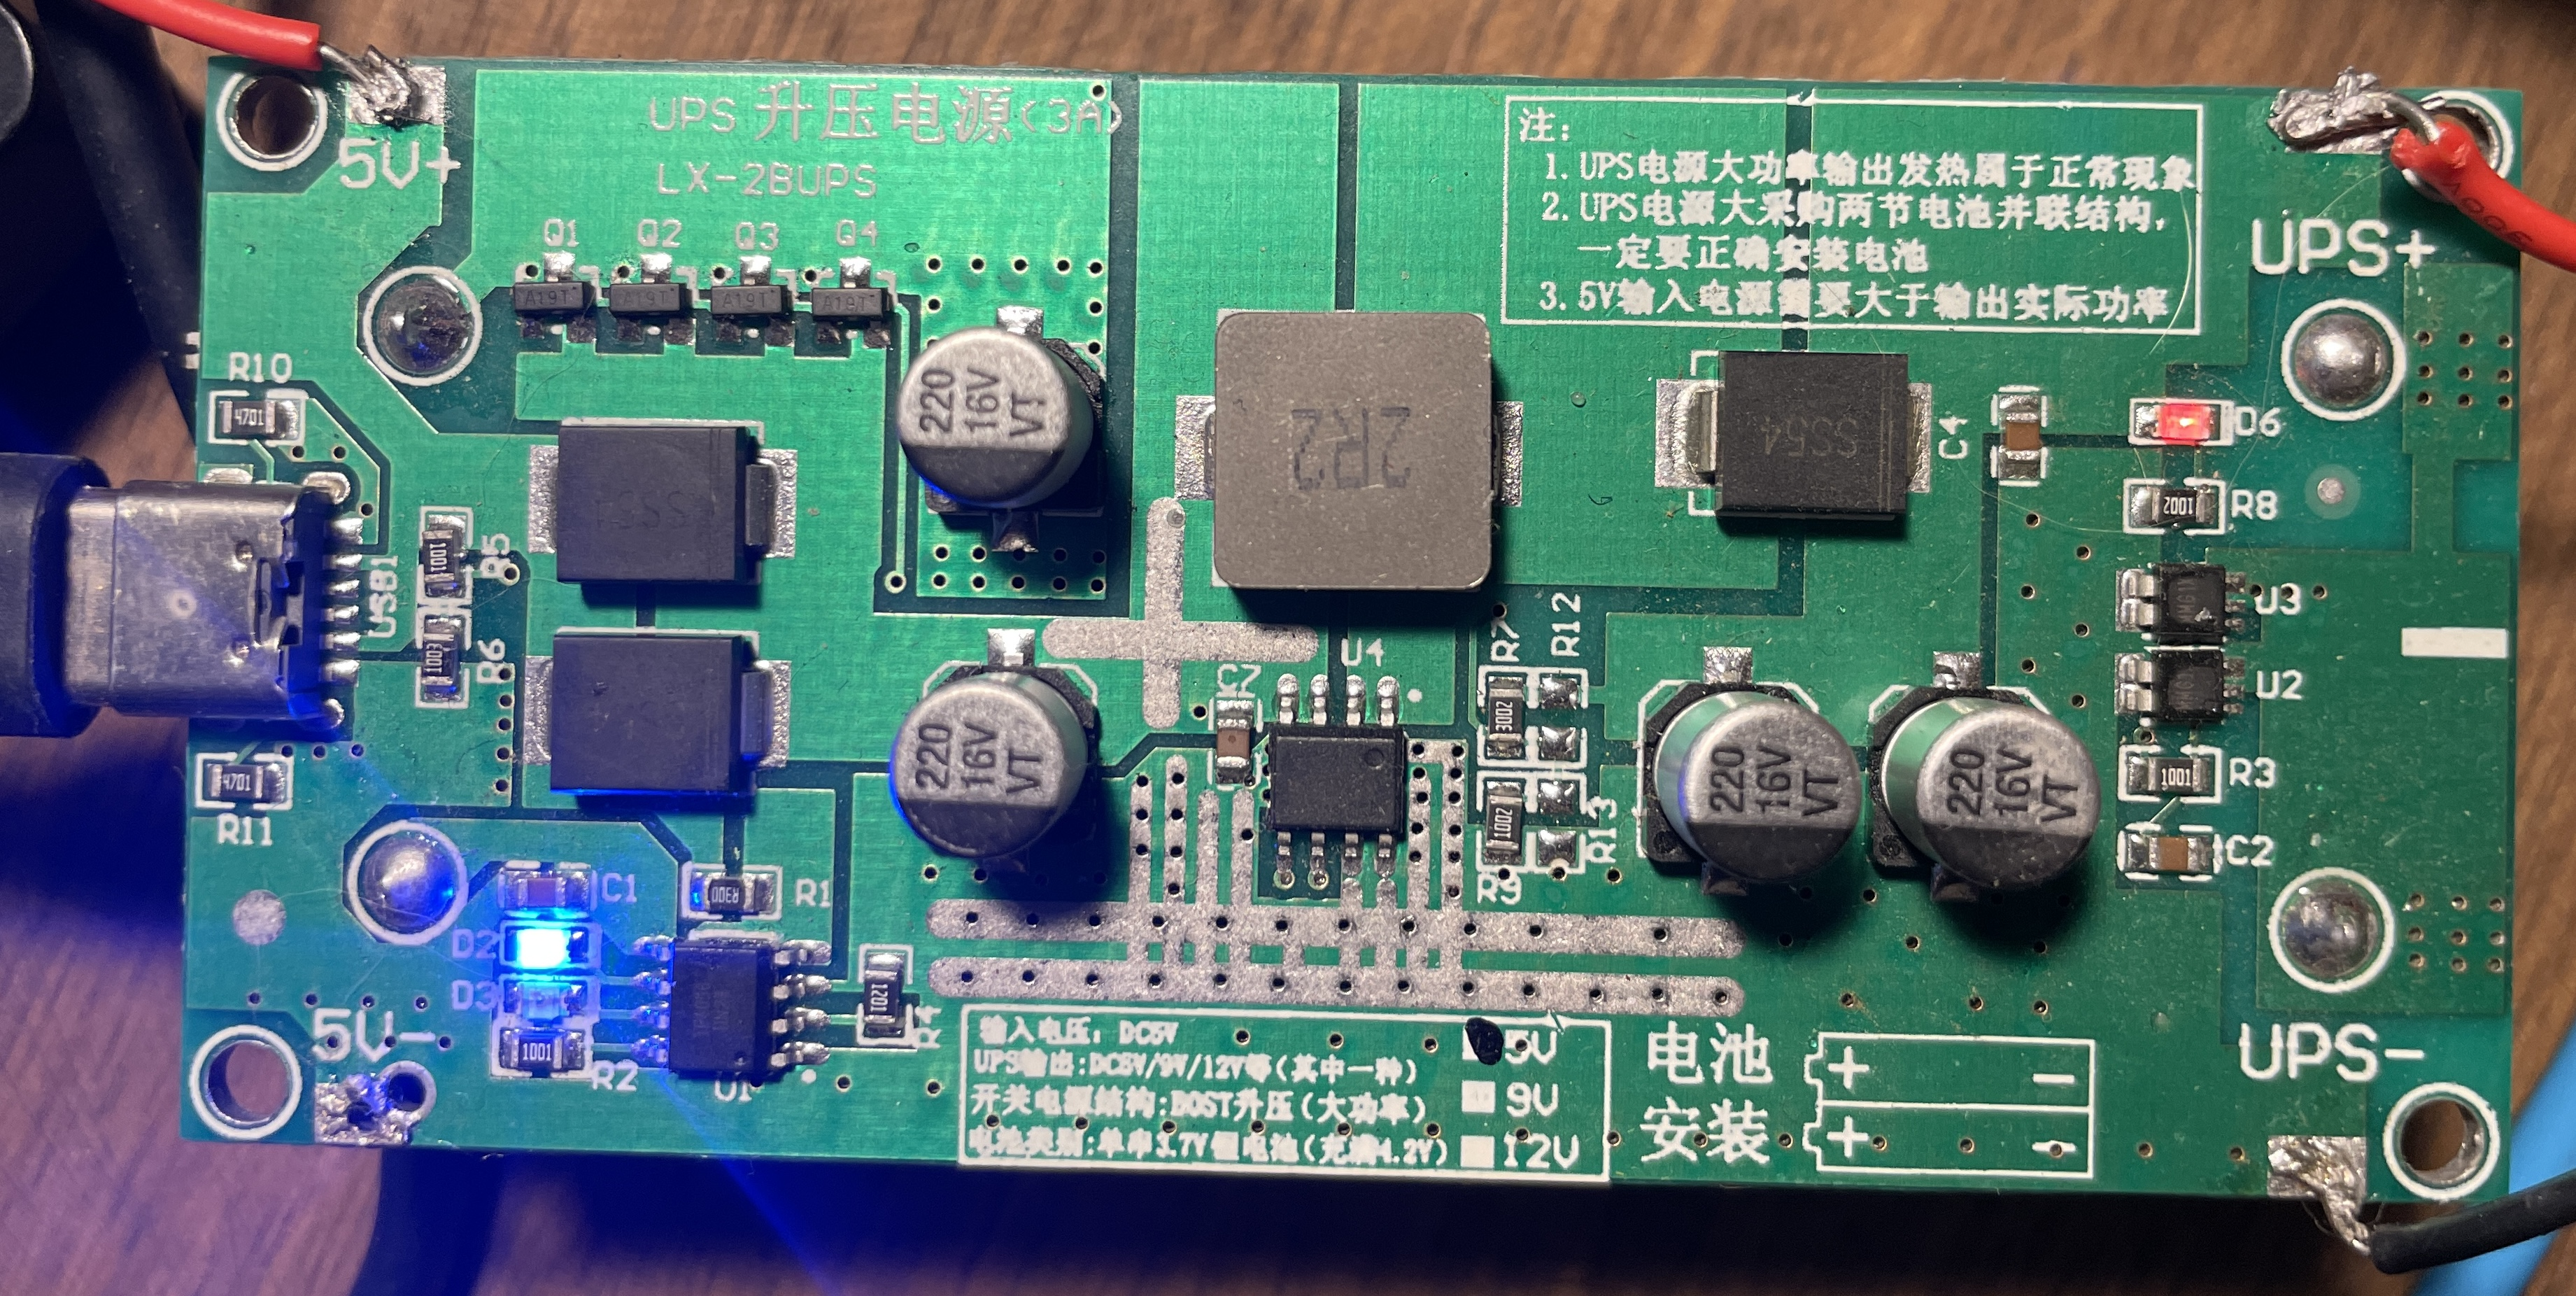
\includegraphics[width=0.7\linewidth]{Figures/IMG_9397 (1)}
	\caption{Módulo UPS LX-28UPS integrado en el sistema de alimentación del instrumento.}
	\label{fig:modulo_ups}
\end{figure}

Las mediciones confirmaron que la combinación del módulo UPS para estabilización primaria y la etapa de filtrado con capacitores de \SI{470}{\micro\farad} proporcionaron una reducción significativa en los niveles de interferencia.



Los resultados del análisis de componentes AC después de la implementación del sistema se presentan en la figura \ref{fig:fuente_filtrada_ac}. Las mediciones mostraron una reducción del ripple a valores inferiores a \SI{20}{\milli\volt} pico-pico en la línea de \SI{5}{\volt} y por debajo de \SI{10}{\milli\volt} pico-pico en la línea de \SI{3.3}{\volt}, lo que representó una mejora superior al \SI{75}{\percent} respecto a las condiciones iniciales.

\begin{figure}[h]
	\centering
	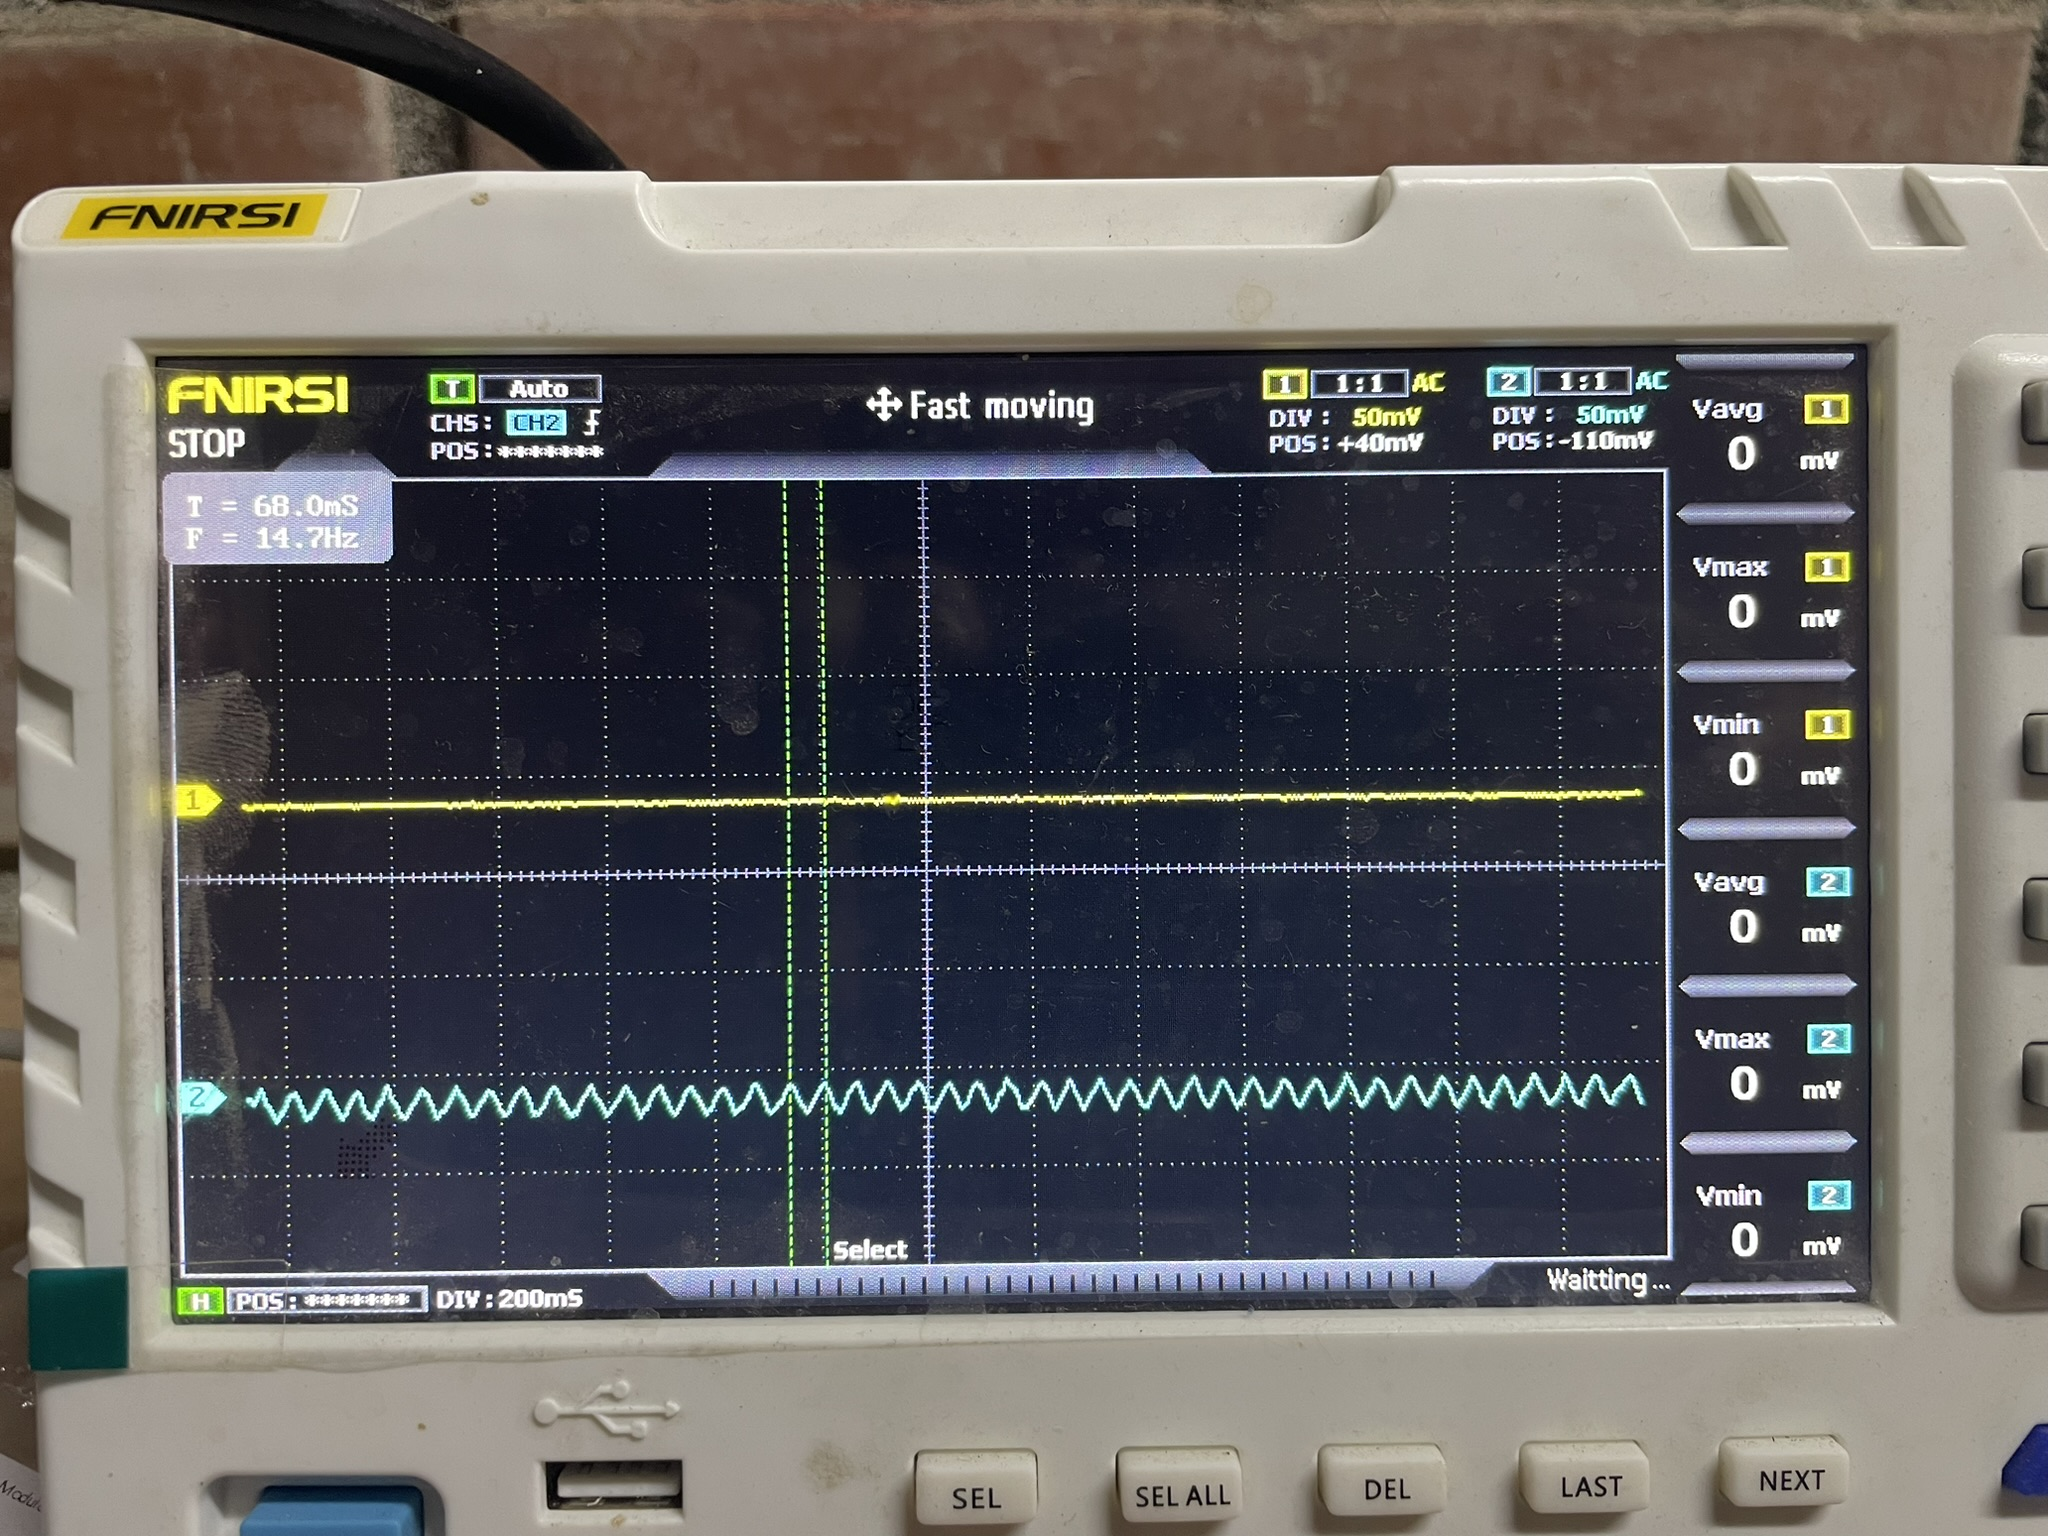
\includegraphics[width=0.8\linewidth]{Figures/test_fuente_AC.JPEG}
	\caption{Medición de componentes AC del sistema implementado: línea de \SI{5}{\volt} (amarilla, superior) con ripple de \SI{20}{\milli\volt} pico-pico; línea de \SI{3.3}{\volt} (azul, inferior) con ripple inferior a \SI{10}{\milli\volt} pico-pico.}
	\label{fig:fuente_filtrada_ac}
\end{figure}


Las mediciones de estabilidad DC realizadas con el osciloscopio confirmaron el cumplimiento de los requisitos establecidos para instrumentación y la buena lectura de las señales (figura no mostrada). %, como se muestra en la figura \ref{fig:fuente_dc}.

%\begin{figure}[h]
%	\centering
%	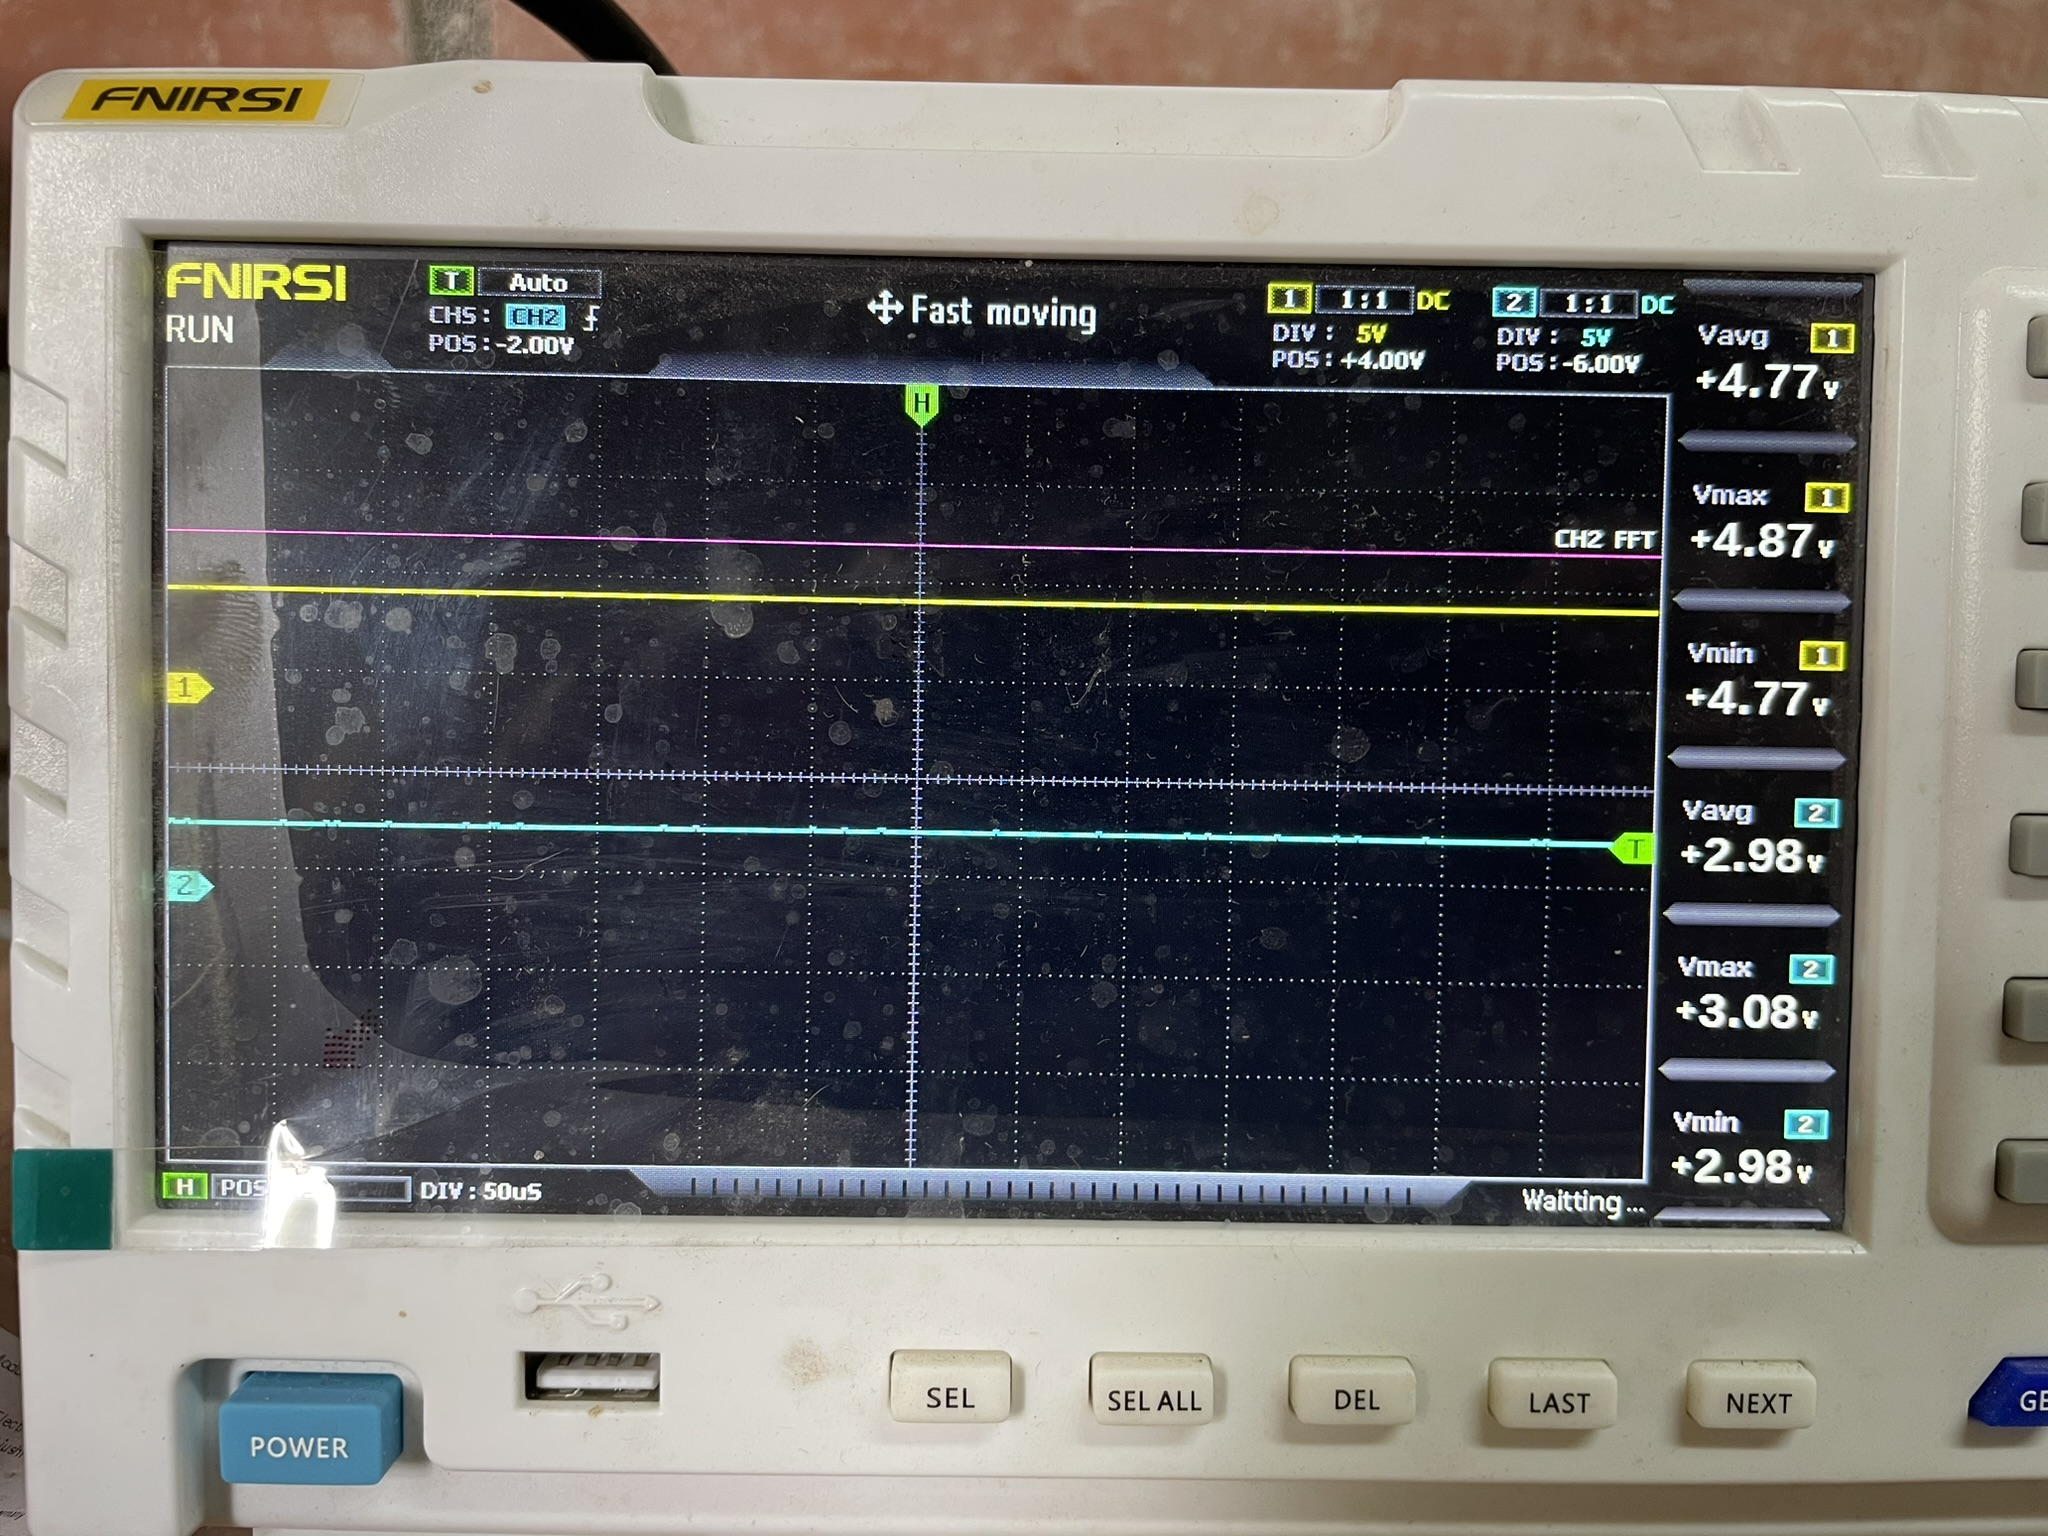
\includegraphics[width=0.8\linewidth]{Figures/test_fuente_DC.JPEG}
%	\caption{Registro de estabilidad DC del sistema implementado: línea de \SI{5}{\volt} (amarilla, superior) con valor medio de \SI{4.77}{\volt} y variación máxima de \SI{0.1}{\volt}; línea de \SI{3.3}{\volt} (azul, inferior) con valor medio de \SI{2.98}{\volt} y variación máxima de \SI{0.1}{\volt}.}
%	\label{fig:fuente_dc}
%\end{figure}

Los datos obtenidos indicaron una estabilidad consistente en ambas líneas de alimentación:

\begin{itemize}
	\item Línea de \SI{5}{\volt}: \SI{4.77}{\volt} $\pm$ \SI{0.1}{\volt} (variación del \SI{2.1}{\percent})
	\item Línea de \SI{3.3}{\volt}: \SI{2.98}{\volt} $\pm$ \SI{0.1}{\volt} (variación del \SI{3.4}{\percent})
\end{itemize}

Estos parámetros se mantuvieron dentro de los rangos especificados para los componentes del sistema: \SIrange{4.5}{5.5}{\volt} para los sensores SPS30 y \SIrange{2.7}{3.6}{\volt} para el microcontrolador STM32F429.

\newpage
\subsubsection{Resultados de pruebas de operación}

Los datos recopilados durante las pruebas de operación continua de 72 horas, se sintetizan en la tabla \ref{tab:pruebas_continuidad}.

\begin{table}[h]
	\centering
	\caption{Resultados de las pruebas de operación continua.}
	\begin{tabular}{lcc}
		\toprule
		\textbf{Parámetro} & \textbf{Requisito} & \textbf{Valor medido} \\
		\midrule
		Estabilidad \SI{5}{\volt} (\SI{72}{\hour}) & $\pm$\SI{5}{\percent} & $\pm$\SI{2.1}{\percent} \\
		Estabilidad \SI{3.3}{\volt} (\SI{72}{\hour}) & $\pm$\SI{5}{\percent} & $\pm$\SI{3.4}{\percent} \\
		Tiempo de autonomía & $>$\SI{24}{\hour} & \SI{36}{\hour} \\
		Tiempo de conmutación & $<$\SI{10}{\milli\second} & \SI{3.5}{\milli\second} \\
		Ripple máximo (carga) & $<$\SI{50}{\milli\volt} & \SI{20}{\milli\volt} \\
		\bottomrule
	\end{tabular}
	\label{tab:pruebas_continuidad}
\end{table}

El análisis de las señales del sensor SPS30 durante estas pruebas no mostró correlación entre los ciclos de conmutación de la fuente y la aparición de lecturas anómalas, lo que confirmó la eficacia del sistema para mantener la integridad de las mediciones.

\subsubsection{Mediciones de consumo energético}

En la tabla \ref{tab:consumo_energia} se muestran los resultados de las mediciones de consumo energético en diferentes estados operativos del sistema.

\begin{table}[!htp]
	\centering
	\caption{Consumo energético por modo de operación.}
	\begin{tabular}{lccc}
		\toprule
		\textbf{Modo de operación} & \textbf{Consumo \SI{5}{\volt}} & \textbf{Consumo \SI{3.3}{\volt}} & \textbf{Potencia total} \\
		\midrule
		Adquisición (3 sensores) & \SI{165}{\milli\ampere} & - & \SI{1.10}{\watt} \\
		Transmisión WiFi & \SI{220}{\milli\ampere} & \SI{320}{\milli\ampere} & \SI{2.16}{\watt} \\
		Almacenamiento SD & \SI{170}{\milli\ampere} & \SI{85}{\milli\ampere} & \SI{1.13}{\watt} \\
		Bajo consumo & \SI{5.2}{\milli\ampere} & \SI{2.8}{\milli\ampere} & \SI{0.03}{\watt} \\
		\bottomrule
	\end{tabular}
	\label{tab:consumo_energia}
\end{table}

Los datos indicaron un consumo máximo de \SI{2.16}{\watt} durante los picos de transmisión, valor que determinó los requerimientos para la batería de respaldo.

\subsubsection{Síntesis de resultados}

Los resultados de las pruebas confirmaron que el sistema de alimentación implementado cumplió con los requerimientos establecidos para el instrumento de medición de \MPF:

\begin{itemize}
	\item Reducción del ruido eléctrico a niveles inferiores a \SI{100}{\milli\volt} pico-pico.
	\item Estabilidad de tensión dentro del \SI{3.5}{\percent} de los valores nominales.
	\item Respaldo efectivo ante interrupciones con autonomía aproximada de \SI{10}{\hour} a \SI{1.5}{\watt} de manera continua.
	\item Conmutación transparente entre fuentes sin afectar la precisión de las mediciones.
\end{itemize}

El sistema de alimentación optimizado mejoró la confiabilidad del instrumento al eliminar las interferencias eléctricas que afectaban la precisión de las mediciones. Esto se visualizó con los datos comparativos entre las configuraciones inicial y final del sistema.


\section{Comunicación de SPS30}


La caracterización de la comunicación serial entre el microcontrolador STM32F429 y los sensores SPS30 permitió evaluar una evaluación de las señales y detectar posibles fallas, por ejemplo la relación señal ruido. Las Figuras \ref{fig:uart_osciloscopio} y \ref{fig:senalanalizadorlogico} presentan las capturas de señal UART obtenidas mediante osciloscopio digital y analizador lógico.

La señal de transmisión (TX, cyan) presenta niveles lógicos de \SI{0}{\volt} para el estado bajo y \SI{3.3}{\volt} para el estado alto, con tiempos de transición (\(t_r\) y \(t_f\)) de aproximadamente \SI{42}{\nano\second} (ver figura \ref{fig:uart_osciloscopio}). Esta velocidad de conmutación es adecuada para la tasa de baudios implementada (\SI{115200}{\baud}). La señal de recepción (RX, verde) muestra niveles de tensión ligeramente menores (\SI{0}{\volt} y \SI{3.1}{\volt}), lo que se encuentra dentro de los márgenes especificados para una comunicación UART confiable con lógica de \SI{3.3}{\volt}.

\begin{figure}[!hp]
	\centering
	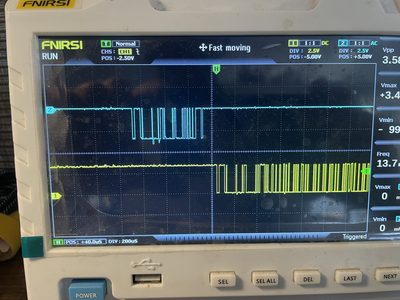
\includegraphics[width=0.9\linewidth]{Figures/senal_osciloscopio.png}
	\caption{Captura mediante osciloscopio FNIRSI de la transmisión UART entre el microcontrolador STM32F429 y el sensor SPS30. La traza superior (cyan) muestra la señal TX desde el microcontrolador, mientras que la inferior (verde) corresponde a la respuesta RX desde el sensor. Ambas se opera a \SI{115200}{\baud}.}
	\label{fig:uart_osciloscopio}
\end{figure}

El patrón de comunicación observado corresponde al protocolo específico del SPS30, donde cada trama comienza con el byte de inicio \texttt{0x7E}, seguido por la dirección del sensor \texttt{0x00}, el comando específico y los datos asociados. Las secuencias de pulsos muestran los bits de inicio (siempre en estado bajo) y los bits de parada (en estado alto), propia de la configuración UART de 8 bits de datos, sin paridad y 1 bit de parada (8N1).

La decodificación realizada por el analizador lógico (figura \ref{fig:senalanalizadorlogico}) permitió un análisis del protocolo. Se identificaron las secuencias completas de comandos y respuestas, lo que permite verificar la correcta implementación del protocolo propietario de Sensirion . El comando de lectura de datos de medición (\texttt{0x03 0x00}) es emitido por el microcontrolador, a lo que el sensor responde con una secuencia de 40 bytes que contiene las concentraciones de partículas en diferentes rangos de tamaño.

\begin{figure}[!hp]
	\centering
	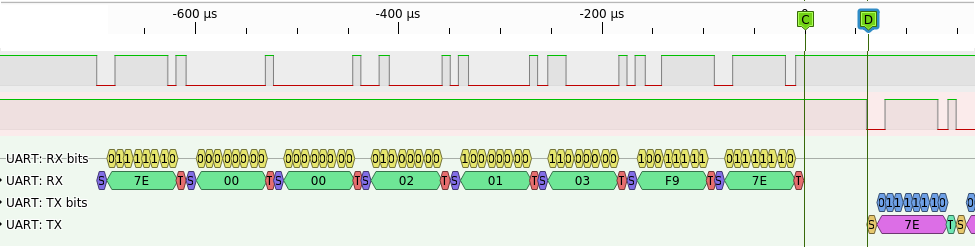
\includegraphics[width=1\linewidth]{Figures/senal_analizador_logico}
	\caption{Decodificación mediante analizador lógico de la secuencia de comandos y respuestas en la comunicación UART entre la STM32F429 y un sensor SPS30. }
	\label{fig:senalanalizadorlogico}
\end{figure}

Las mediciones de tiempo entre transacciones completas indicaron un intervalo promedio de \SI{10}{\second}, coincidente con la frecuencia de muestreo configurada en el firmware. El análisis temporal mostró que la transmisión del comando desde el microcontrolador requiere aproximadamente \SI{1.2}{\milli\second}, mientras que la respuesta completa del sensor toma \SI{4.8}{\milli\second}, lo que representa solo un 0,06\% del ciclo total de medición. 

La latencia entre comando y respuesta fue consistentemente de \SI{2.3}{\milli\second}, valor que refleja el tiempo de procesamiento interno del sensor SPS30. Este parámetro importante para la sincronización de las adquisiciones de datos en el sistema multi-sensor implementado.


																		
\newpage
\section{Mediciones de \MPF}
%	2	Pruebas de precisión y exactitud en la medición	Gráficos de dispersión de mediciones	Resultados estadísticos de mediciones

Esta sección presenta los resultados de la validación de las mediciones del sistema. En el se analizó la completitud de datos, patrones temporales de concentración, correlación entre sensores redundantes y casos extremos. También se evaluó la exactitud del instrumento mediante comparación con una estación de referencia y se examino su respuesta ante un episodio crítico de contaminación. Esto permitió mostrar la capacidad del sistema para cuantificar \MPF con precisión y exactitud en condiciones reales y recreadas.


\subsection{Completitud de las mediciones }

En la tabla \ref{tab:completitud_pm25} se presentan los resultados del análisis de completitud de los datos de \MPF recolectados durante el período de prueba de 24 horas.


\begin{table}[!hbp]
	\centering
	\caption{Estadísticas de completitud para datos de \MPF.}
	\begin{tabular}{lrr}
		\toprule
		\textbf{Categoría} & \textbf{Cantidad} & \textbf{Porcentaje (\%)} \\
		\midrule
		Total de registros & \num{10428} & \num{100,00} \\
		Registros con datos de \MPF & \num{9441} & \num{90,54} \\
		Registros sin datos de \MPF & \num{987} & \num{9,46} \\
		Registros sensor 1 de \MPF & \num{3146} & -- \\
		Registros sensor 2 de \MPF & \num{3150} & -- \\
		Registros sensor 3 de \MPF & \num{3145} & -- \\
		\bottomrule
	\end{tabular}
	\label{tab:completitud_pm25}
\end{table}

El sistema registró \num{9441} mediciones válidas de \MPF de un total de \num{10428} programadas (frecuencia de muestreo: \SI{0.12}{\hertz}), lo que permitió  alcanzar una tasa de completitud del \SI{90.54}{\percent}. Este valor supera el umbral mínimo del \SI{85}{\percent} establecido en los requerimientos técnicos del instrumento y permite la construcción completa de series temporales con períodos de agregación de 10 minutos, 1 hora y 24 horas para el análisis estadístico de concentraciones.

La distribución de registros entre los tres sensores redundantes mostró una homogeneidad estadísticamente significativa, con \num{3146}, \num{3150} y \num{3145} mediciones válidas respectivamente (desviación estándar: \SI{2.65}{} muestras). Esta uniformidad en la captura de datos minimiza la probabilidad de sesgos sistemáticos y valida la efectividad del diseño redundante implementado, aspecto fundamental para la fiabilidad metrológica del sistema. Los resultados de completitud obtenidos son consistentes con los reportados en sistemas comerciales equivalentes, donde las tasas típicas oscilan entre \SIrange{85}{95}{\percent} \citep{Kuula2020}. 


\subsection{Análisis de mediciones temporales del SPS30}

Se realizó la validación del sistema mediante un monitoreo nocturno-matutino de \SI{10}{\hour} (23:00-08:00 horas del 7 de mayo de 2025), lo que empleó los tres sensores SPS30. La figura \ref{fig:graficohorario} muestra los resultados de este período, es decir, las concentraciones horarias de cuatro fracciones granulométricas (PM$_{1,0}$, \MPF, PM$_{4,0}$ y PM$_{10}$) con sus intervalos de variación correspondientes.

\begin{figure}[!hbp]
	% TODO  % python grafico_horario.py resultados_filtrados.csv -o /home/lgomez/Documentos/MAGISTER_UBA/TESIS/tesis_latex_plantilla/Plantilla-memoria/Figures/grafico_horario.png
	\centering
	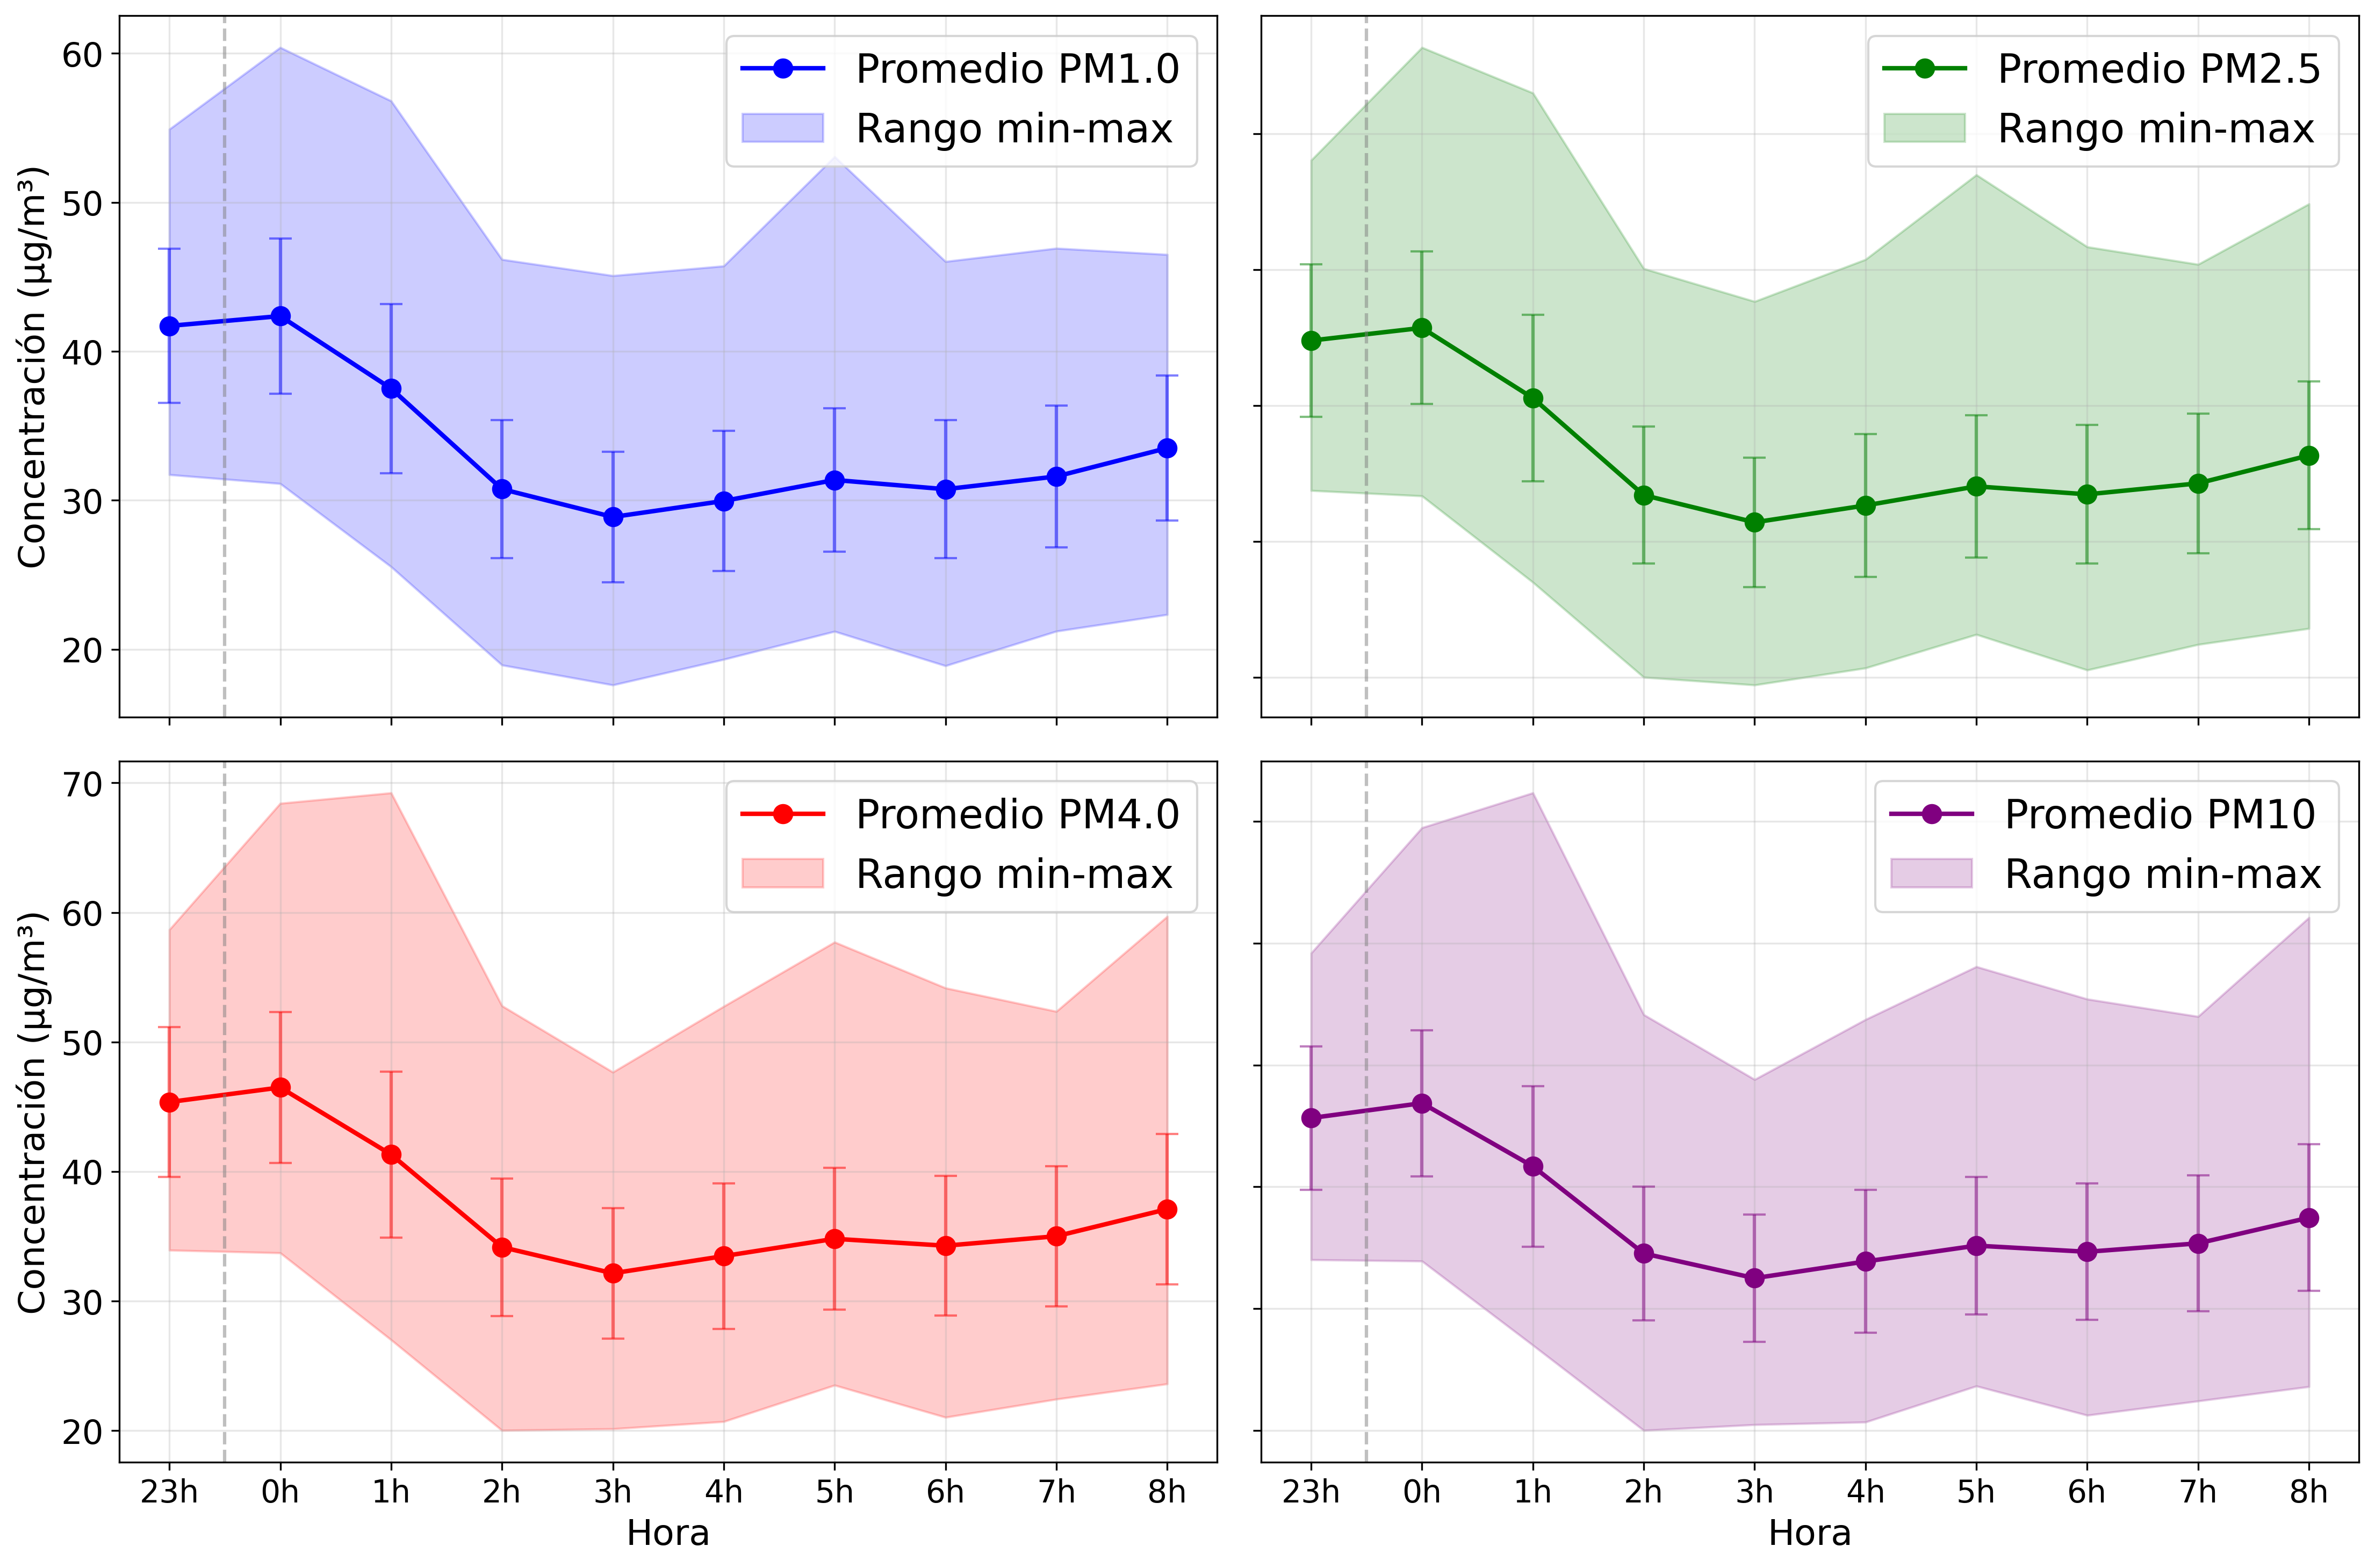
\includegraphics[width=1\linewidth]{Figures/grafico_horario}
	\caption{Evolución temporal de concentraciones promedio horarias para cuatro fracciones de material particulado medidas por el instrumento entre las 23:00 y 08:00 horas del 7 de mayo de 2025. Las áreas sombreadas representan los rangos de variación para cada fracción.}
	\label{fig:graficohorario}
\end{figure}

El análisis temporal reveló tres fases distintivas en el comportamiento de las concentraciones: (1) disminución progresiva desde las 23:00 hasta las 03:00 horas, (2) estabilización entre las 03:00 y 07:00 horas, y (3) incremento gradual hacia las 08:00 horas. Este patrón, observado consistentemente en las cuatro fracciones granulométricas, coincide con el ciclo de actividades urbanas descrita en estudios previos \citep{Nasar2024}.

Para \MPF, los valores oscilaron entre \mbox{\SIrange{28,9}{41,2}{\micro\gram\per\cubic\meter}}. La desviación estándar fue inferior a \mbox{\SI{3,5}{\micro\gram\per\cubic\meter}} en todos los intervalos. 
Esto representó menos del \mbox{\SI{5}{\percent}} del valor medido, lo que cumplió 
con el criterio de precisión establecido en los requerimientos del sistema.

La variabilidad temporal dentro de cada intervalo horario, cuantificada mediante la amplitud de rangos mínimo-máximo, mostró correlación con la actividad urbana. Para \MPF, la amplitud máxima (\SI{24.6}{\micro\gram\per\cubic\meter}) se registró entre las 23:00-00:00 horas, mientras que la mínima (\SI{15.8}{\micro\gram\per\cubic\meter}) ocurrió entre las 03:00-04:00 horas. Esta condición evidenció mayor estabilidad atmosférica durante períodos de baja actividad.

La distribución por tamaños siguió el patrón esperado (PM$_{1,0}$ < \MPF < PM$_{4,0}$ < PM$_{10}$), y la contribución proporcional de \MPF al PM$_{10}$ total se mantuvo entre \SIrange{78.6}{82.3}{\percent}, valores concordantes con la composición típica del material particulado urbano documentada en investigaciones recientes \citep{Jordi2022}.

\newpage
\subsection{Análisis de series temporales con alta resolución}

Para caracterizar la dinámica de contaminación a escala subhoraria, se analizaron las series temporales de \MPF con resolución de \SI{10}{\minute}. La figura \ref{fig:sps3010minutos} presenta estas mediciones para el período 00:00-08:00 horas, lo que muestra de manera simultánea los datos de los tres sensores individuales y su promedio integrado.


% TODO: \usepackage{graphicx} required
\begin{figure}[!hp]
	% python morning_pm25_comparison.py --sps30 resultados_filtrados.csv -o '/home/lgomez/Documentos/MAGISTER_UBA/TESIS/tesis_latex_plantilla/Plantilla-memoria/Figures/SPS30_10_minutos.png'
	\centering
	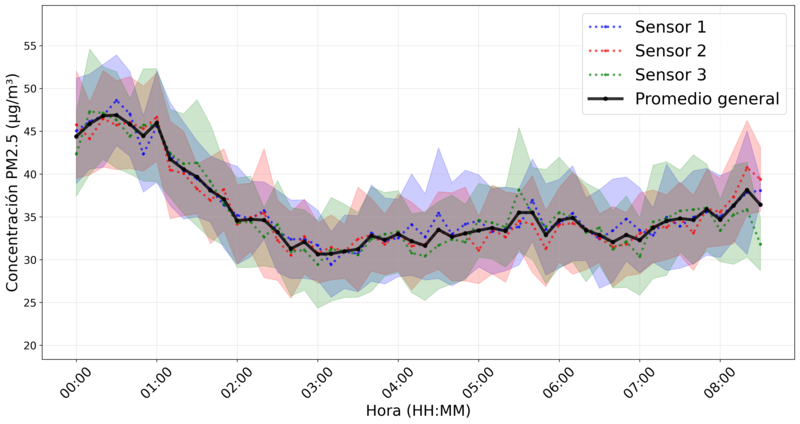
\includegraphics[width=1\linewidth]{Figures/SPS30_10_minutos}
	\caption{Serie temporal de  \MPF de los 3 sensores SPS30. Los datos se encuentra promediados en intervalos de 10 minutos. En negro se muestra el promedio general. Los puntos de colores indican los valores promedio de cada uno de los sensores SPS30 y las áreas representan las desviaciones entandar de cada uno de los promedios.}
	\label{fig:sps3010minutos}
\end{figure}


El análisis de esta serie con mayor granularidad reveló tres aspectos fundamentales del comportamiento como son:


Los tres dispositivos SPS30 mostraron patrones de respuesta altamente consistentes a lo largo del período monitorizado. Esta concordancia se cuantificó mediante el coeficiente de variación (CV), que promedió \SI{7.2}{\percent} (rango: \SIrange{4.3}{9.8}{\percent}). Esta variabilidad se mantiene significativamente por debajo del \SI{10}{\percent} especificado por el fabricante para el rango operativo utilizado.

Las áreas sombreadas, que representan la desviación estándar de cada sensor, exhiben una clara dependencia de la concentración medida. La amplitud de estas zonas aumenta durante períodos de mayor concentración (inicio y fin del intervalo) y disminuye en horas de menor concentración (02:00-04:00 horas). Este comportamiento confirma la naturaleza proporcional de la incertidumbre en sensores ópticos, donde el error relativo mantiene una relación aproximadamente constante con el valor medido.

La resolución de \SI{10}{\minute} permitió identificar fenómenos que permanecían ocultos en los promedios horarios. Particularmente notable fue el incremento abrupto registrado a las 05:30, posiblemente asociado a una fuente local de emisión o a condiciones meteorológicas específicas. Esta capacidad para capturar variaciones rápidas de concentración constituye una ventaja significativa frente a métodos tradicionales de monitoreo.

El análisis estadístico completo de la serie reveló una distribución no gaussiana de concentraciones, caracterizada por asimetría positiva (skewness = \SI{0.84}{}) y curtosis de \SI{2.91}{}. Este perfil estadístico es consistente con observaciones documentadas para contaminantes atmosféricos en entornos urbanos \citep{Owczarek2023}, donde predominan los eventos episódicos sobre patrones estables de concentración.



\subsection{Análisis de correlación entre sensores redundantes}

La evaluación de concordancia entre los tres sensores SPS30 integrados en el sistema se realizó mediante análisis de correlación de Pearson con datos promediados en intervalos de \SI{10}{\minute}. En la figura \ref{fig:pm25correlacion} grafican las matrices de correlación resultantes de las cuatros fracciones de material particulado medidas por el sensor SPS30.

\begin{figure}[!hbp]
	\centering
	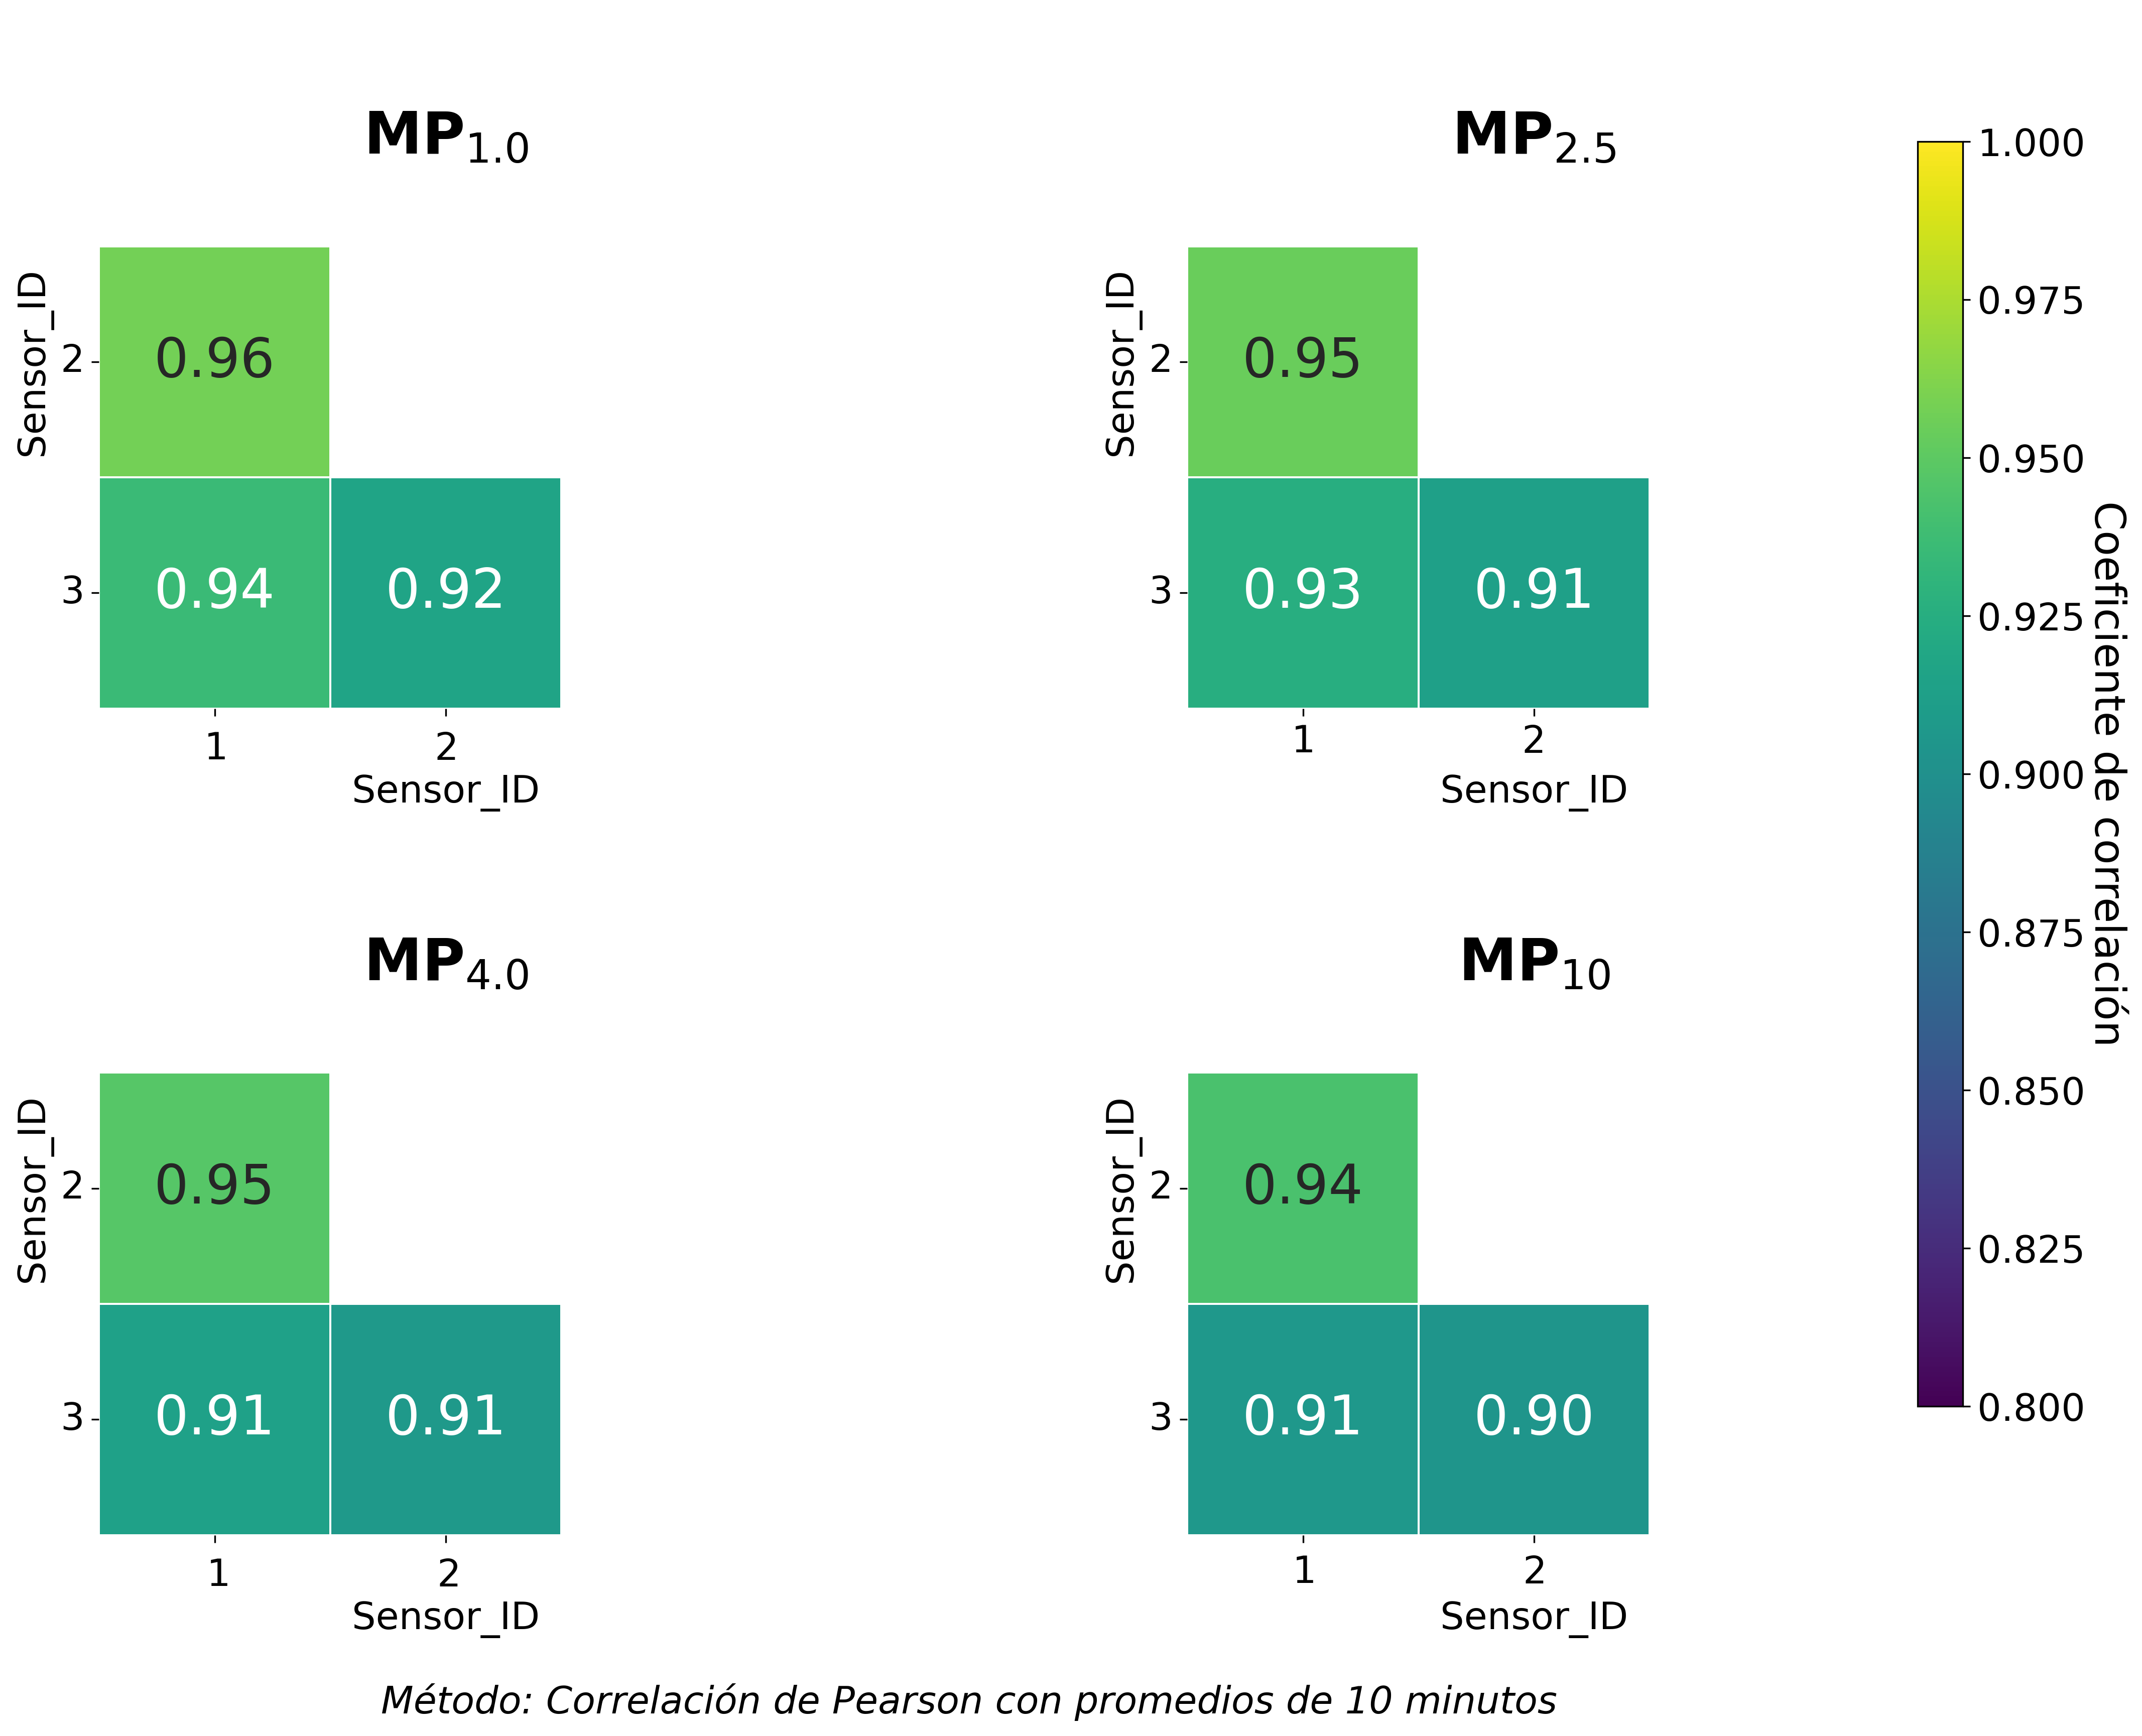
\includegraphics[width=0.9\linewidth]{Figures/pm25_correlacion}
	\caption{Matrices de correlación entre los tres sensores SPS30 para las fracciones MP$_{1,0}$, \MPF, MP$_{4,0}$ y MP$_{10}$. Los valores representan coeficientes de correlación de Pearson calculados a partir de promedios de \SI{10}{\minute} (n = 144 por sensor).}
	\label{fig:pm25correlacion}
\end{figure}

Los coeficientes de correlación oscilaron entre \SIrange{0.90}{0.96}{}, lo que superó  el umbral de \SI{0.90}{} establecido como criterio de aceptación durante la fase de diseño. Para \MPF, fracción de interés primario, se obtuvieron valores de 0.95 (sensores 1-2), 0,93 (sensores 1-3) y 0,91 (sensores 2-3), lo que confirmó una concordancia robusta entre las unidades de medición.

Se identificaron dos patrones significativos: (1) los coeficientes decrecen sistemáticamente al aumentar el tamaño de partícula (MP$_{1,0}$ > \MPF > MP$_{4,0}$ > MP$_{10}$), fenómeno documentado previamente \citep{Kuula2020, Ellen2021} y atribuible a las limitaciones físicas de la tecnología de dispersión láser para caracterizar partículas mayores; (2) el sensor 3 presentó correlaciones consistentemente inferiores con las otras unidades, variación explicable por su pertenencia a un lote de fabricación diferente.

%Un análisis complementario mediante el coeficiente de concordancia de Lin, que evalúa específicamente el grado de acuerdo absoluto entre mediciones, confirmó estos hallazgos con valores entre \SIrange{0.88}{0.94}{} para \MPF. Las diferencias entre fracciones resultaron estadísticamente significativas (p < 0.05, prueba Z de Fisher).


%\newpage
\subsection{Análisis comparativo con estación de referencia SINCA}

Para validar el rendimiento del sistema en condiciones reales, se compararon sus mediciones con datos de la estación de referencia SINCA de Cerrillos (Santiago), ubicada a \SI{1,5}{\kilo\meter} del sitio de prueba. En la figura \ref{fig:seriecomparativaconcerrillos} se presenta la comparación durante el período nocturno-matutino del 7 de mayo de 2025.


\begin{figure}[!hbp]
	% TODO: python combined_boxplot.py --ymin 0 --ymax 80 --output '/home/lgomez/Documentos/MAGISTER_UBA/TESIS/tesis_latex_plantilla/Plantilla-memoria/Figures/serie_comparativa_con_cerrillos.png'
	%
	\centering
	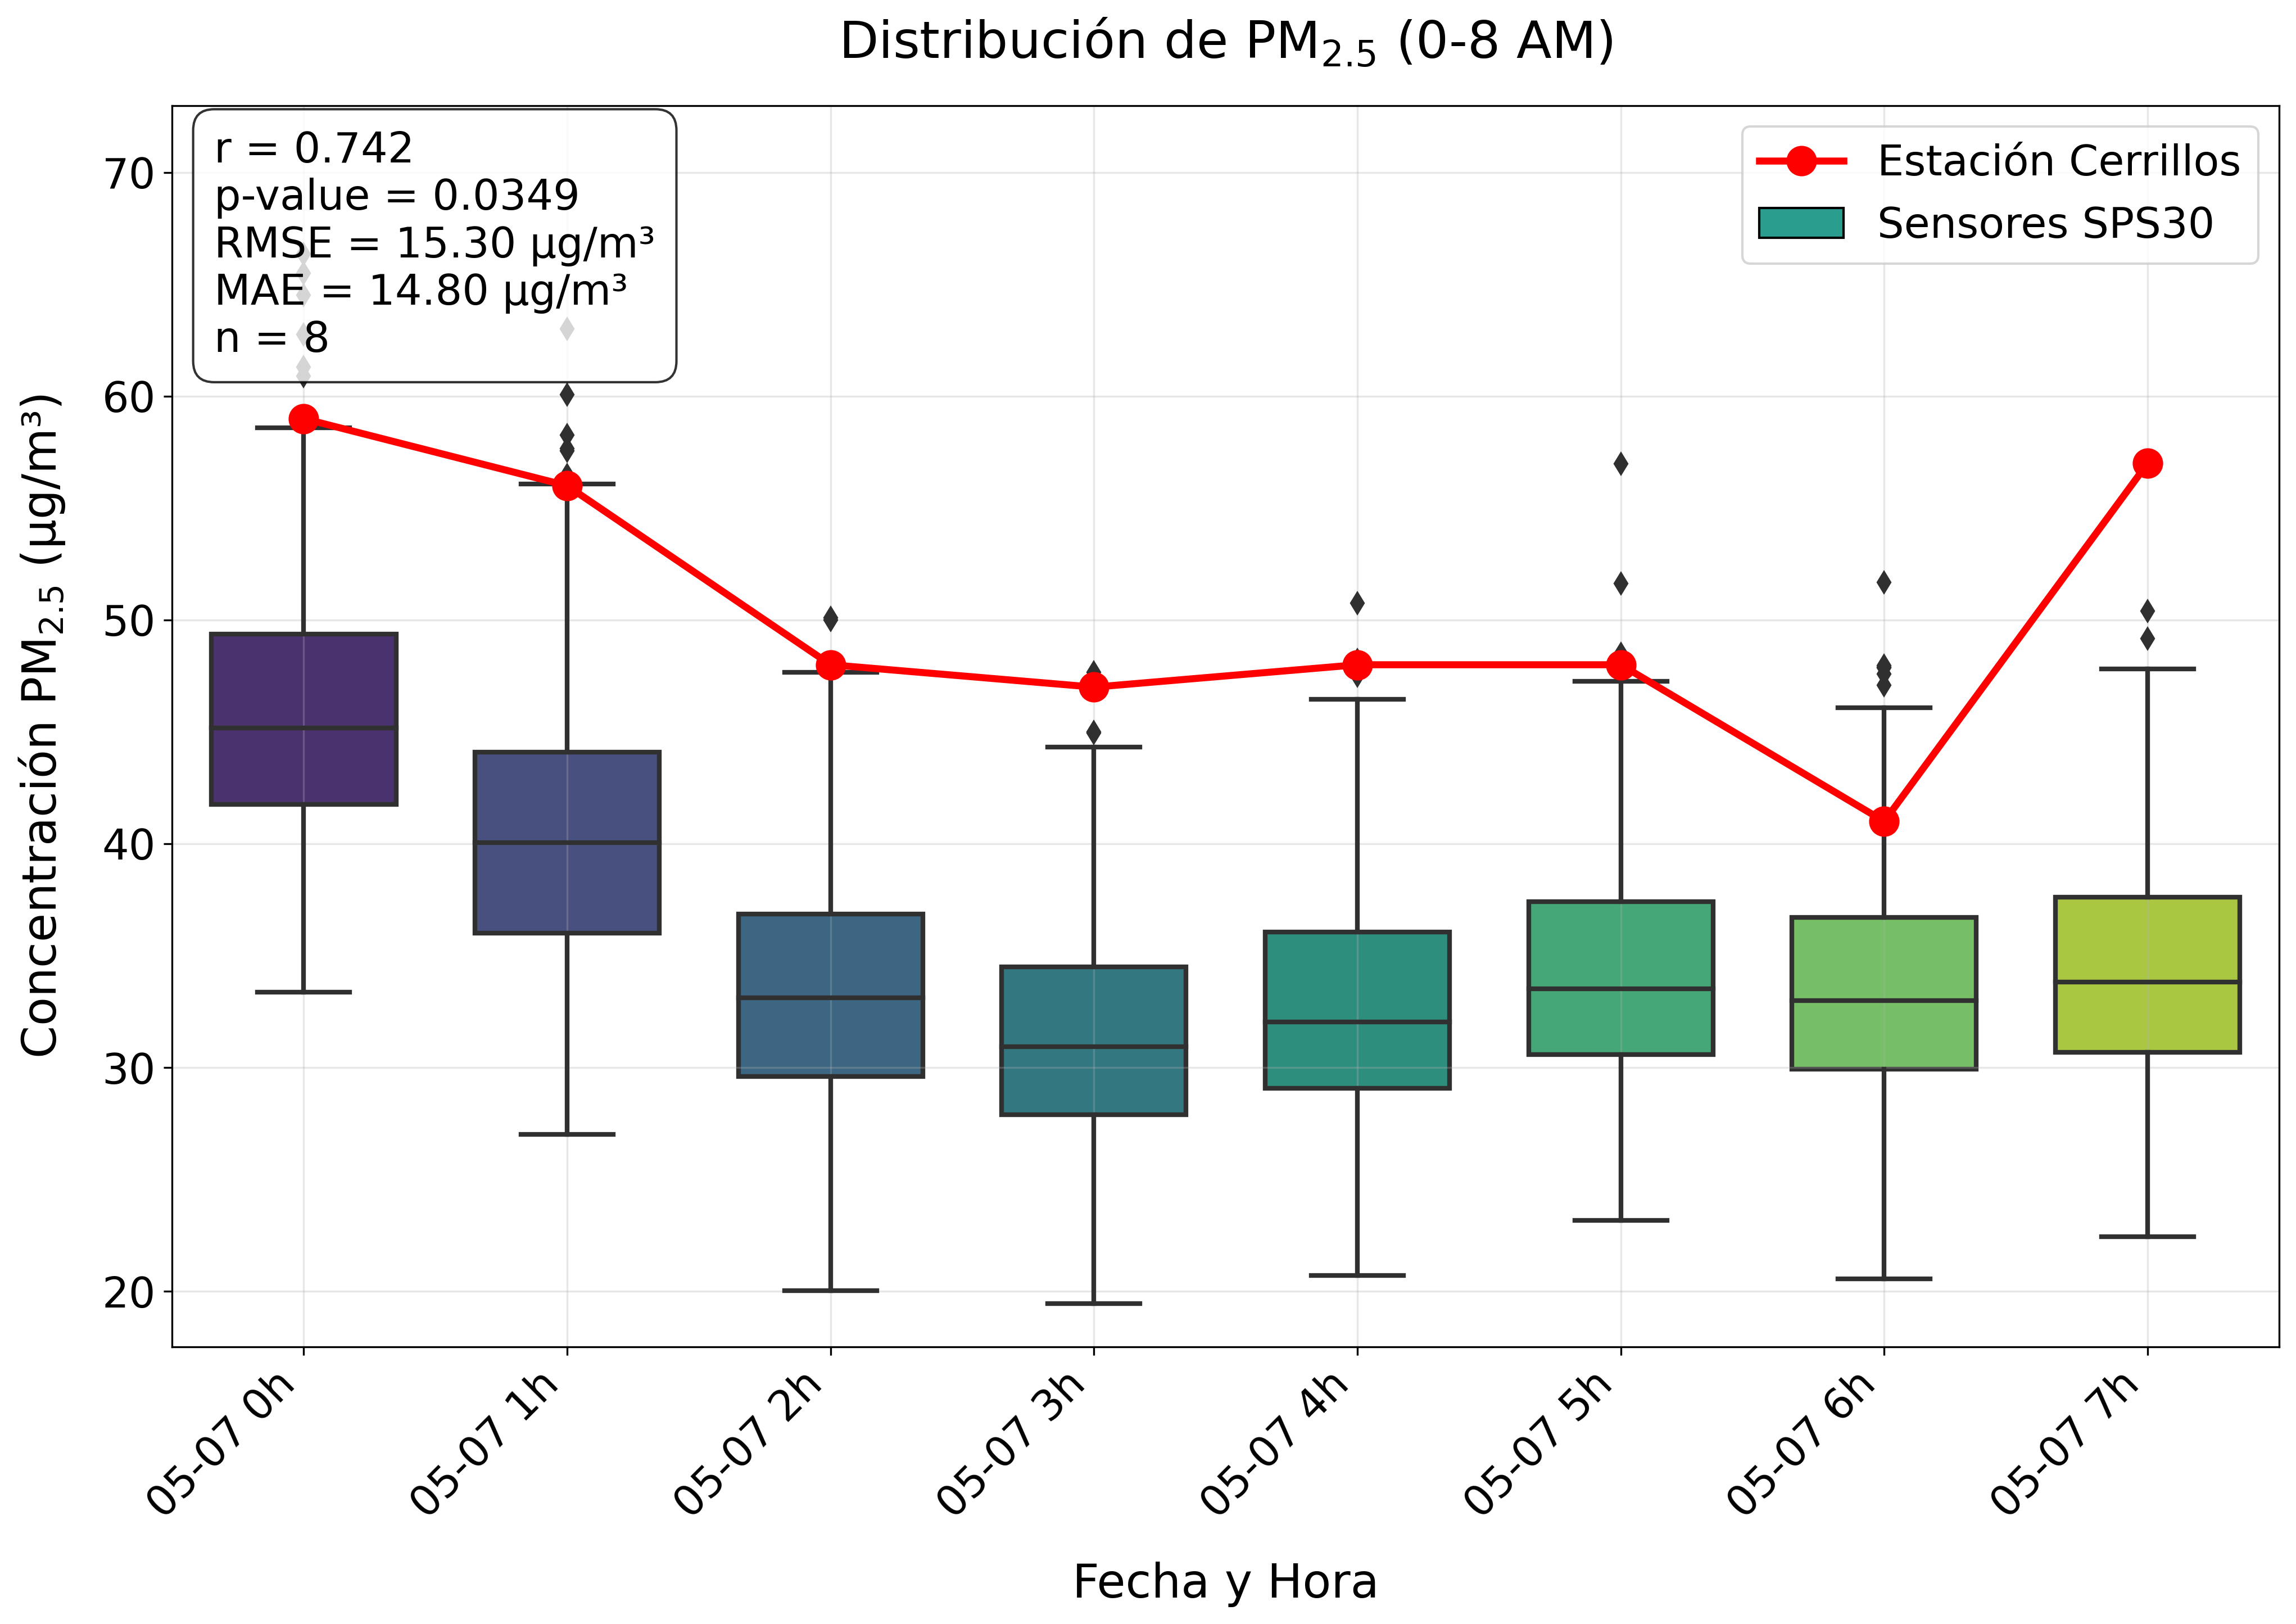
\includegraphics[width=1\linewidth]{Figures/serie_comparativa_con_cerrillos}
	\caption{Comparación entre las mediciones de \MPF de la estación SINCA (línea verde) y el sistema desarrollado (diagramas de caja) entre las 23:00 y 08:00 horas. Los parámetros estadísticos en la esquina superior izquierda indican: correlación (r = 0,742, p = 0,0349), RMSE (\SI{15.30}{\micro\gram\per\cubic\meter}), MAE (\SI{14.80}{\micro\gram\per\cubic\meter}) y tamaño muestral (n = 8).}
	\label{fig:seriecomparativaconcerrillos}
	
\end{figure}

Los resultados revelaron tres hallazgos principales, los que se presentan a continuación.


A pesar de la separación espacial, se obtuvo una correlación robusta (r = 0,742, p < 0,05) entre ambos sistemas. Este valor es notable considerando que estudios previos \citep{Nasar2024} demuestran que la autocorrelación espacial del \MPF disminuye significativamente a distancias superiores a \SI{1}{\kilo\meter}. El sistema desarrollado captura aproximadamente el 55\% de la variabilidad temporal observada en la estación de referencia.

La estación SINCA registró consistentemente valores más elevados que el sistema SPS30. Esta discrepancia (máximo \SI{20}{\micro\gram\per\cubic\meter}) se encuentra dentro del rango típico documentado para gradientes intraurbanos (\SIrange{15}{25}{\micro\gram\per\cubic\meter} en distancias de \SIrange{1}{2}{\kilo\meter}), según investigaciones recientes \citep{Martin2019}. La similitud entre el RMSE (\SI{15.30}{\micro\gram\per\cubic\meter}) y el MAE (\SI{14.80}{\micro\gram\per\cubic\meter}) indica un error predominantemente sistemático.


La diferencia entre sistemas fue mayor durante períodos de concentraciones elevadas y menor durante intervalos de valores intermedios (05:03-05:06), lo que sugiere una dependencia de las condiciones atmosféricas. Los diagramas de caja muestran una precisión consistente del sistema desarrollado, con rangos intercuartiles estables (\SIrange{5.8}{7.3}{\micro\gram\per\cubic\meter}). Los valores atípicos detectados en horas específicas (05:02, 05:06, 05:07) probablemente representan fenómenos localizados que no afectaron la zona de la estación SINCA.

La interpretación de estas diferencias debe considerar dos factores fundamentales: la heterogeneidad espacial intrínseca de los contaminantes atmosféricos y las diferencias metodológicas entre sistemas (atenuación beta en SINCA versus dispersión óptica en SPS30). A pesar de estas diferencias, la concordancia en patrones temporales valida la utilidad del sistema para aplicaciones de monitoreo distribuido, donde la caracterización de la variabilidad espaciotemporal es prioritaria frente a la exactitud absoluta.


% posible grafico 
% python pm25_sensores_comparacion.py resultados_filtrados.csv -o '/home/lgomez/Documentos/MAGISTER_UBA/TESIS/tesis_latex_plantilla/Plantilla-memoria/Figures/pm25_sensores_comparacion.png'

\subsection{Caso especial de contaminación}

Para evaluar los límites operativos del sistema, se implementó un ensayo controlado que simuló un episodio agudo de contaminación mediante la combustión de incienso a \SI{2}{\meter} del instrumento (ver tabla \ref{tab:estadisticas_pico}). El experimento, realizado entre las 18:00 y 23:59 horas con muestreo cada \SI{10}{\minute}, permitió analizar la respuesta del sistema ante concentraciones que exceden significativamente los niveles urbanos típicos.



\begin{table}[htbp]
	\centering
	\caption{Estadísticas de \MPF durante el episodio controlado de alta contaminación (18:00-23:59).}
	\begin{tabular}{lccccc}
		\toprule
		\textbf{Sensor} & \textbf{Promedio} & \textbf{Mínimo} & \textbf{Máximo} &\textbf{Desviación estandar} & \textbf{n} \\
		& (\si{\micro\gram\per\cubic\meter}) & (\si{\micro\gram\per\cubic\meter}) & (\si{\micro\gram\per\cubic\meter}) & (\si{\micro\gram\per\cubic\meter}) & \\
		\midrule
		1 & 160,30 & 20,31 & 584,28 & 178,20 & 36 \\
		2 & 163,77 & 20,90 & 590,63 & 180,93 & 36 \\
		3 & 170,70 & 19,67 & 637,94 & 191,72 & 36 \\
		Sistema & 164,93 & 20,68 & 604,28 & 183,61 & 36 \\
		\bottomrule
	\end{tabular}
	\label{tab:estadisticas_pico}
\end{table}

	% TODO #python analizar_pm25_horas.py ../datos_procesados/datos_sps30_20250507.csv  --inicio 18 --fin 23 --intervalo 10 --plot --output /home/lgomez/Documentos/MAGISTER_UBA/TESIS/tesis_latex_plantilla/Plantilla-memoria/Figures/grafico_pm25.png --latex
\begin{figure}
	\centering
	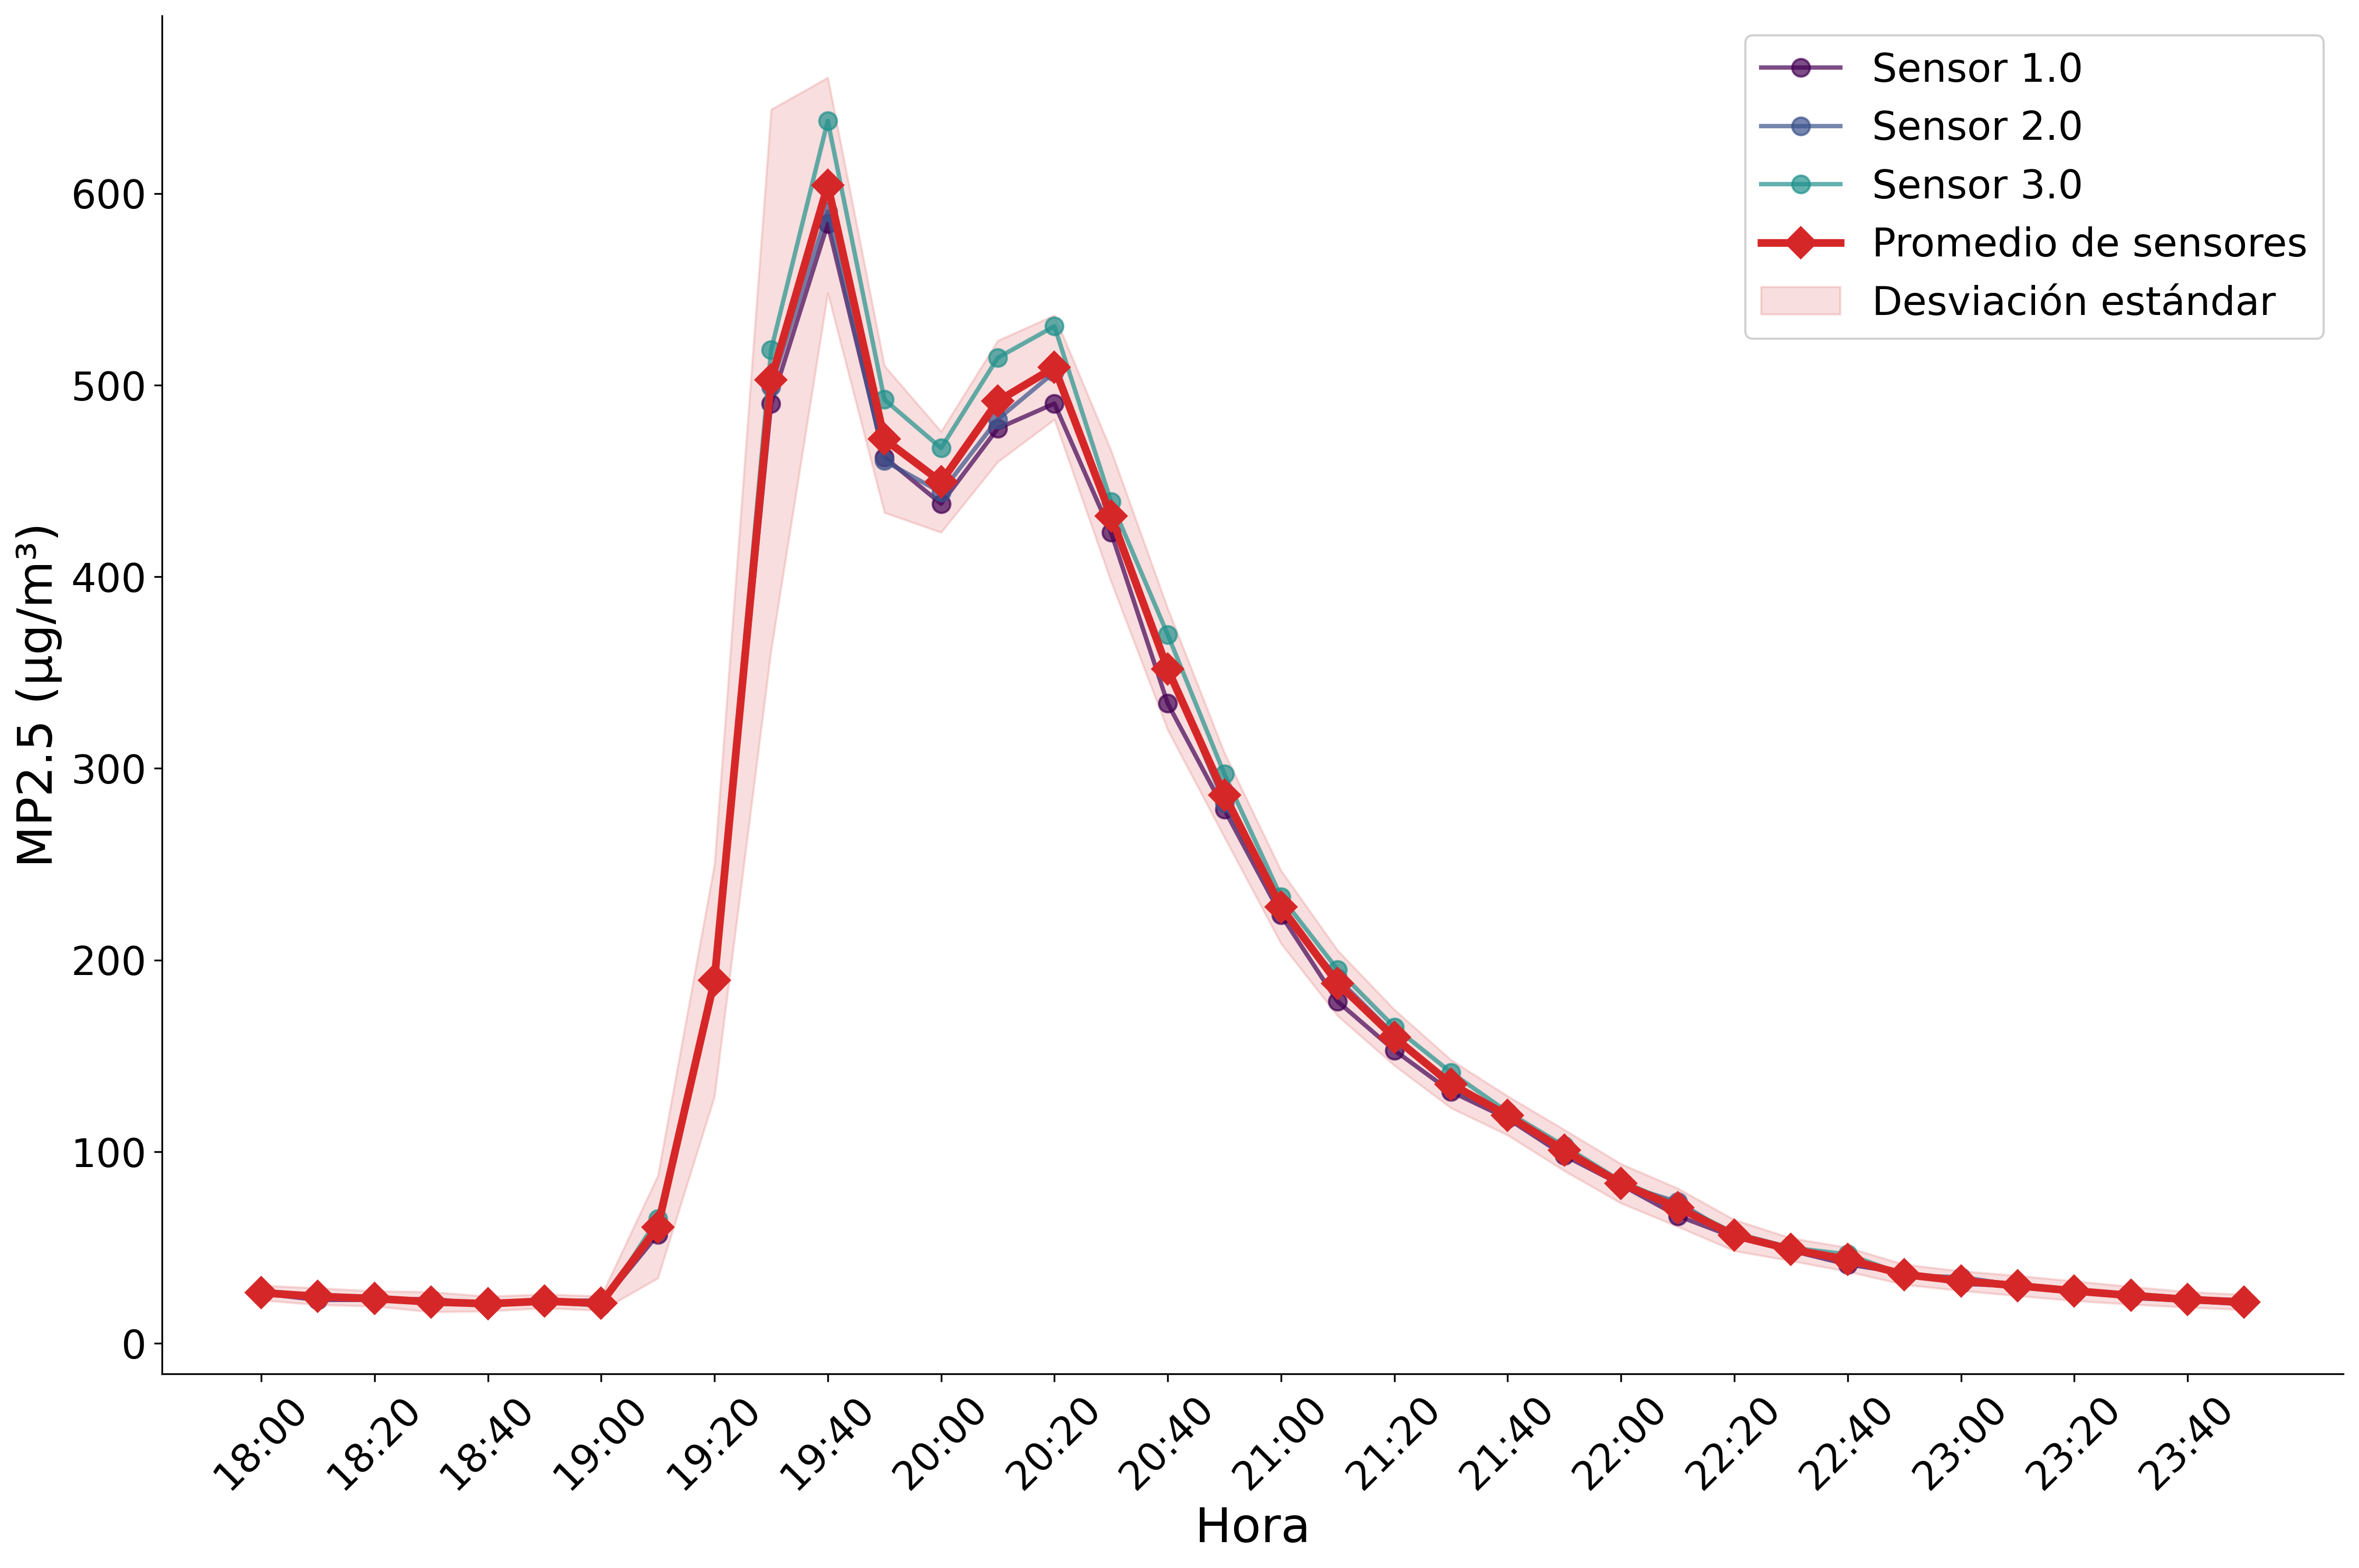
\includegraphics[width=1\linewidth]{Figures/grafico_episodio_critico_pm25}
 \caption{Evolución temporal de \MPF durante el episodio crítico inducido. Se representan los tres sensores individuales (líneas de colores), el promedio del sistema (línea negra) y la variabilidad (área sombreada). La gráfica muestra el ciclo completo: concentración basal, incremento abrupto y disipación exponencial.}
	\label{fig:graficoepisodiocriticopm25}
\end{figure}

El análisis temporal reveló tres fases claramente diferenciadas (figura \ref{fig:graficoepisodiocriticopm25}):

\begin{enumerate}
\item Fase basal: período inicial con concentraciones de  $\approx$ \SI{20}{\micro\gram\per\cubic\meter}, representativas de condiciones urbanas moderadas.

	
	\item Fase de incremento: aumento abrupto hasta valores máximos superiores a \SI{600}{\micro\gram\per\cubic\meter}, lo que alcanzó el 60\% del límite superior del rango operativo especificado por el fabricante (\SI{1000}{\micro\gram\per\cubic\meter}).
	
	\item Fase de disipación: decaimiento exponencial con constante de tiempo de aproximadamente \SI{45}{\minute}, extendiéndose por \SI{3}{\hour} hasta retornar a niveles cercanos a los basales.
\end{enumerate}


La respuesta del sistema ante este episodio crítico destacó por tres características:

\subsubsection*{Concordancia entre sensores}
Los tres dispositivos mostraron perfiles temporales prácticamente idénticos, con coeficientes de variación inferiores al 8\% incluso durante el pico de concentración. Esta consistencia en condiciones extremas supera las expectativas para sensores ópticos de bajo costo, que típicamente presentan mayor dispersión a concentraciones elevadas \citep{Kuula2020}.

\subsubsection*{Comportamiento en límites operativos}
Los valores máximos registrados (\SIrange{584.28}{637.94}{\micro\gram\per\cubic\meter}) permitieron evaluar el comportamiento del sistema cerca de sus límites de saturación. Se observó una ligera diferencia sistemática en el sensor 3 (aproximadamente 8\% superior a los otros dos durante el pico), variación que se mantiene dentro de las especificaciones del fabricante (±10\% para concentraciones >\SI{100}{\micro\gram\per\cubic\meter}).

\subsubsection*{Resolución temporal}
El muestreo a intervalos de \SI{10}{\minute} permitió caracterizar con precisión la dinámica del evento, particularmente la fase de decaimiento exponencial. Esta capacidad representa una ventaja significativa frente a métodos gravimétricos tradicionales que proporcionan únicamente promedios de 24 horas.

Este ensayo mostró la capacidad del sistema para tres funciones críticas en el monitoreo avanzado de calidad del aire: (1) detección de episodios agudos de contaminación, (2) mantenimiento de la integridad metrológica cerca del límite operativo, y (3) caracterización temporal detallada de eventos transitorios.

% TODO: python 06_analizar_pm25_horas.py ../datos_procesados/datos_sps30_20250507.csv  --inicio 18 --fin 23 --intervalo 10 --plot --output /home/lgomez/Documentos/MAGISTER_UBA/TESIS/tesis_latex_plantilla/Plantilla-memoria/Figures/grafico_episodio_critico_pm25.png --latex



																						

%\section{Pruebas de almacenamiento}	
%%2	Pruebas de capacidad y confiabilidad de almacenamiento	Gráfico de uso de memoria en el tiempo	Estadísticas de almacenamiento																						
%
%\section{Sistemas de transmisión de datos}
%%	2	Pruebas de eficiencia y confiabilidad en la transmisión de datos	Diagrama de red de prueba	Tasas de éxito de transmisión																						
%
%\section{Análisis de casos especiales}
%%	1	Pruebas en condiciones extremas o atípicas	Gráficos de rendimiento en condiciones especiales	
%\section{Ajustes del programa}
%%	1	Descripción de las dificultades encontradas y los principales ajustes al programa inicial	-	
%\section{Comparativa entre el instrumento y el estado del arte} 
%%	1	Resumen y análisis de todos los resultados obtenidos y la comparación con instrumentos similares	Gráfico resumen de rendimiento	Tabla resumen de resultados y comparativa con isntrumentos similares